\documentclass[letterpaper,10pt]{book}
% Change to 10 pt
\usepackage{pdfpages}
\usepackage{morewrites}			% to counteract the no write space problem
\setcounter{tocdepth}{5}

\usepackage[framemethod=TikZ]{mdframed}

\usepackage{fancyhdr}

\usepackage{paralist}
\usepackage{amsmath}
\usepackage{amsfonts}
\usepackage{amssymb}
\usepackage{graphicx}

\usepackage{datetime}
%\usepackage{ulem}

%\usepackage[nottoc]{toobibind}

\usepackage[inline]{enumitem}

% Outer margin at 2.50 is exactly correct to fit the ``corruption alert'' tables
\usepackage[inner=1.0in, outer=2.50in, top=2.54cm,bottom=2.54cm, marginparwidth=2.25in]{geometry}

\usepackage{marginnote}
\usepackage{longtable}
\usepackage{booktabs}
\usepackage{xcolor}

\usepackage{soul}

\usepackage{marginnote}
\usepackage{imakeidx} 
\usepackage[
	backref=true,
	style=numeric,
%	citestyle=numeric,
	backend=bibtex
	]{biblatex}
\usepackage[driverfallback=hypertex,colorlinks=True]{hyperref}
\usepackage{cleveref}

\makeindex[name=scripture,columnsep=20pt, columnseprule=True,columns=3, title=Scripture References]
\makeindex[name=speaker,columnsep=20pt, columnseprule=True,,columns=2, title=Sermon Creator]
\makeindex[name=series,columnsep=20pt, columnseprule=True,,columns=2, title=Sermon Series]
\makeindex[name=date,columnsep=20pt, columnseprule=True,columns=2, title=Sermon Date]

\makeindex[name=event,columnsep=20pt, columnseprule=True,columns=2, title=Event]

\makeindex[name=topic,columnsep=20pt, columnseprule=True,columns=2, title=Topic]
\makeindex[name=AWIP,columnsep=20pt, columnseprule=True,columns=3, title=All Words in Passage]
\makeindex[name=NWIV,columnsep=20pt, columnseprule=True,columns=3, title=Number of Words in Verse]
\makeindex[name=PNIP,columnsep=20pt, columnseprule=True,columns=3, title=Proper Names in Passage]
\makeindex[name=PEIP,columnsep=20pt, columnseprule=True,columns=2, title=Prophetic Events in Passage]


\makeindex[name=TWPAQ,columnsep=20pt, columnseprule=True,columns=1, title=13-Word Phrases and Quotes]
\makeindex[name=PFTTIS,columnsep=20pt, columnseprule=False,columns=3, title=Phrases found 13 times in scripture]
\makeindex[name=WFTTIS,columnsep=20pt, columnseprule=False,columns=3, title=Words found 13 times in scripture]
\makeindex[name=WFITV,columnsep=20pt, columnseprule=False,columns=3, title=Words found in exactly 13 verses]
\makeindex[name=EVENTS,columnsep=20pt, columnseprule=False,columns=2, title=Sermon Log by Place]
\makeindex[name=QUESTIONS,columnsep=20pt, columnseprule=False,columns=2, title=Bible Questions]

\makeindex[name=DOCTRINES,columnsep=20pt, columnseprule=False,columns=2, title=Doctrines]

\makeindex[name=SONGS,columnsep=20pt, columnseprule=False,columns=1, title=Songs]
\makeindex[name=LOCATION,columnsep=20pt, columnseprule=False,columns= 2, title=Location]
\makeindex[name=FACEBOOK,columnsep=20pt, columnseprule=False,columns=2, title=Facebook]

\makeindex[name=DEVOTIONAL,columnsep=20pt, columnseprule=False,columns=1, title=Devotionals]

\pagestyle{fancy}
\fancyhf{}
\fancyhead[LE,RO]{\today}
\fancyhead[RE,LO]{Notes, Outlines, Comments}
\fancyhead[CE,CO]{-page \thepage  - }

\fancyfoot[CO,CE]{\leftmark}
%\fancyfoot[LE,RO]{CSCE 692, HW1}

\title{DBR\\
Daily \\ Reads}
\author{Keith Anthony \\
\today }
%\title

%+/ffffff +   \pagenumbering{gobble}

\bibliography{Bibliographies/All20220108}

%%%%% TWEAKS:
%%% - distance from fcolorbox frame to text
\setlength{\fboxsep}{1.0pt}

\usepackage[utf8]{inputenc}
\usepackage{tikz}

%%%%%%%%%%%%%%%%%%%%%%%%%%%%%%%%%%%%%%%%%%%%%%%%%%%%%%%%%%%%%%%%%%%%%%%%%%%%%%%%

\begin{document}

\begin{titlepage}

% Set the text of the page to right-aligned until \end{flushright}
\begin{flushright}
\rightskip=-2.5cm

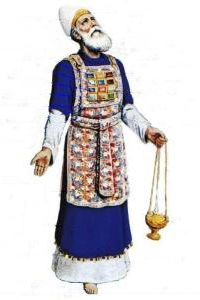
\includegraphics[width=50mm,scale=1.5]{Melchisedec.jpg}
\vspace{0.4in}

% Create a title for the document and write it in bold font
\LARGE{\textbf{\date}}
\linebreak

\vspace{0.5in}


\begin{flushleft}
\LARGE{Psalms 26-50 (Volume II)\\}\vspace{0.25in}
\LARGE{Notes, Outlines, Comments}
\end{flushleft}

% write in large letters
%\large{Free webservices and apps}

% Skip some space
\vspace{0.6in}

%\large{Documentation}
% Skip some space

\bigskip

\normalsize{Xenia, Oh.\\}
\normalsize{updated: \today}

% Skip some space
\vspace{1.3in}

\end{flushright}
% End the title page
\end{titlepage}

%\titlehttps://www.overleaf.com/project/60d732302fc633866943c9d2JE

\newpage 

\tableofcontents\hypertarget{TOC}{}
\listoffigures
\listoftables

\hyphenation{A-bim-e-lech bre-thren E-phra-im  Gib-e-o-nites Jer-u-sa-lem through-out Phil-i-stines The-o-phil-us Am-a-le-kites ven-geance Mesh-el-e-mi-ah onan-ism Phar-a-oh Py-thon thoughts grev-ous-ness Hach-a-liah adul-ter-er Shad-rach}

%\fcolorbox{black}{bone}{TEXT}
%%%%%%%%%%%%%%%%% EXTRA COLORS
%%%%%%%%%%%%%%%%% EXTRA COLORS
%%%%%%%%%%%%%%%%% EXTRA COLORS
\definecolor{champagne}{rgb}{0.97,0.91,0.81}
\definecolor{bone}{rgb}{0.89,0.85,0.79}

\definecolor{ForestGreen}{rgb}{0.00,0.29,0.098}
\definecolor{GIVING}{cmyk}{1,0.0,0.72,.1}

\definecolor{MLPE}{cmyk}{1,1,0,.45}
\definecolor{SOCCER}{cmyk}{.77, 0, .42, .49}
\definecolor{PAYBILL}{cmyk}{0,0.83,0.76,0.07}
\definecolor{SERMON}{cmyk}{.14,.9,0,.30} % aka seance \href{http://www.flatuicolorpicker.com/purple-cmyk-color-model/}{seance}
\definecolor{BIBLE}{cmyk}{0,.17,.74,.17}
\definecolor{WORKBLUE}{cmyk}{1, .5, 0, .6}
\definecolor{myOrange}{cmyk}{0, .4, .98, .03}
\definecolor{myTan}{cmyk}{0.0,.07,.17,.10}
\definecolor{myRed}{cmyk}{0,1,1,0}
\definecolor{myWhite}{cmyk}{0,0,0,0}
\definecolor{BLUESoD}{cmyk}{.97,.84,0,.04}
\definecolor{WHITE}{cmyk}{0,0,0,0}
\definecolor{OLDGOLD}{cmyk}{0.05,0.3,1.00,0}
\definecolor{CASTLETON}{cmyk}{1,0,0.31,0.66}
\definecolor{cadmiumgreen}{rgb}{0.0, 0.42, 0.24}
\definecolor{jungle}{rgb}{0.203,0.4882,0.1718}
\definecolor{MYGOLD}{rgb}{1,.84,0}

\definecolor{MYLIGHTGRAY}{rgb}{.85,.85,.85}

\definecolor{codegreen}{rgb}{0,0.6,0}
\definecolor{codegray}{rgb}{0.5,0.5,0.5}
\definecolor{codepurple}{rgb}{0.58,0,0.82}
\definecolor{backcolour}{rgb}{0.95,0.95,0.92}



\mdfdefinestyle{MyFrame}{%
    linecolor=blue,
    outerlinewidth=2pt,
    roundcorner=5pt,
    innertopmargin=\baselineskip,
    innerbottommargin=\baselineskip,
    innerrightmargin=10pt,
    innerleftmargin=10pt,
    backgroundcolor=gray!25!white}


\mdfdefinestyle{MyFrame2}{%
    linecolor=black,
    outerlinewidth=2pt,
    roundcorner=5pt,
    innertopmargin=\baselineskip,
    innerbottommargin=\baselineskip,
    innerrightmargin=10pt,
    innerleftmargin=10pt,
    backgroundcolor=yellow!25!white}



%\input{PFTTIS}
%\input{WFTTIS}
%\input{WFITV}

%
%\newpage
%\begin{figure}
%\begin{center}
%\includegraphics[scale=.7, angle=0]{05OT-Deuteronomy/References/AndrewSmithDeuteronomyTimeline.png}
%\caption[Deuteronomy Timeline by Andrew Smith]{Deuteronomy Timeline by Andrew %Smith}
%\label{fig:Deuteronomy Timeline by Andrew Smith}
%\end{center}
%\end{figure}

\newpage
\begin{figure}
\begin{center}
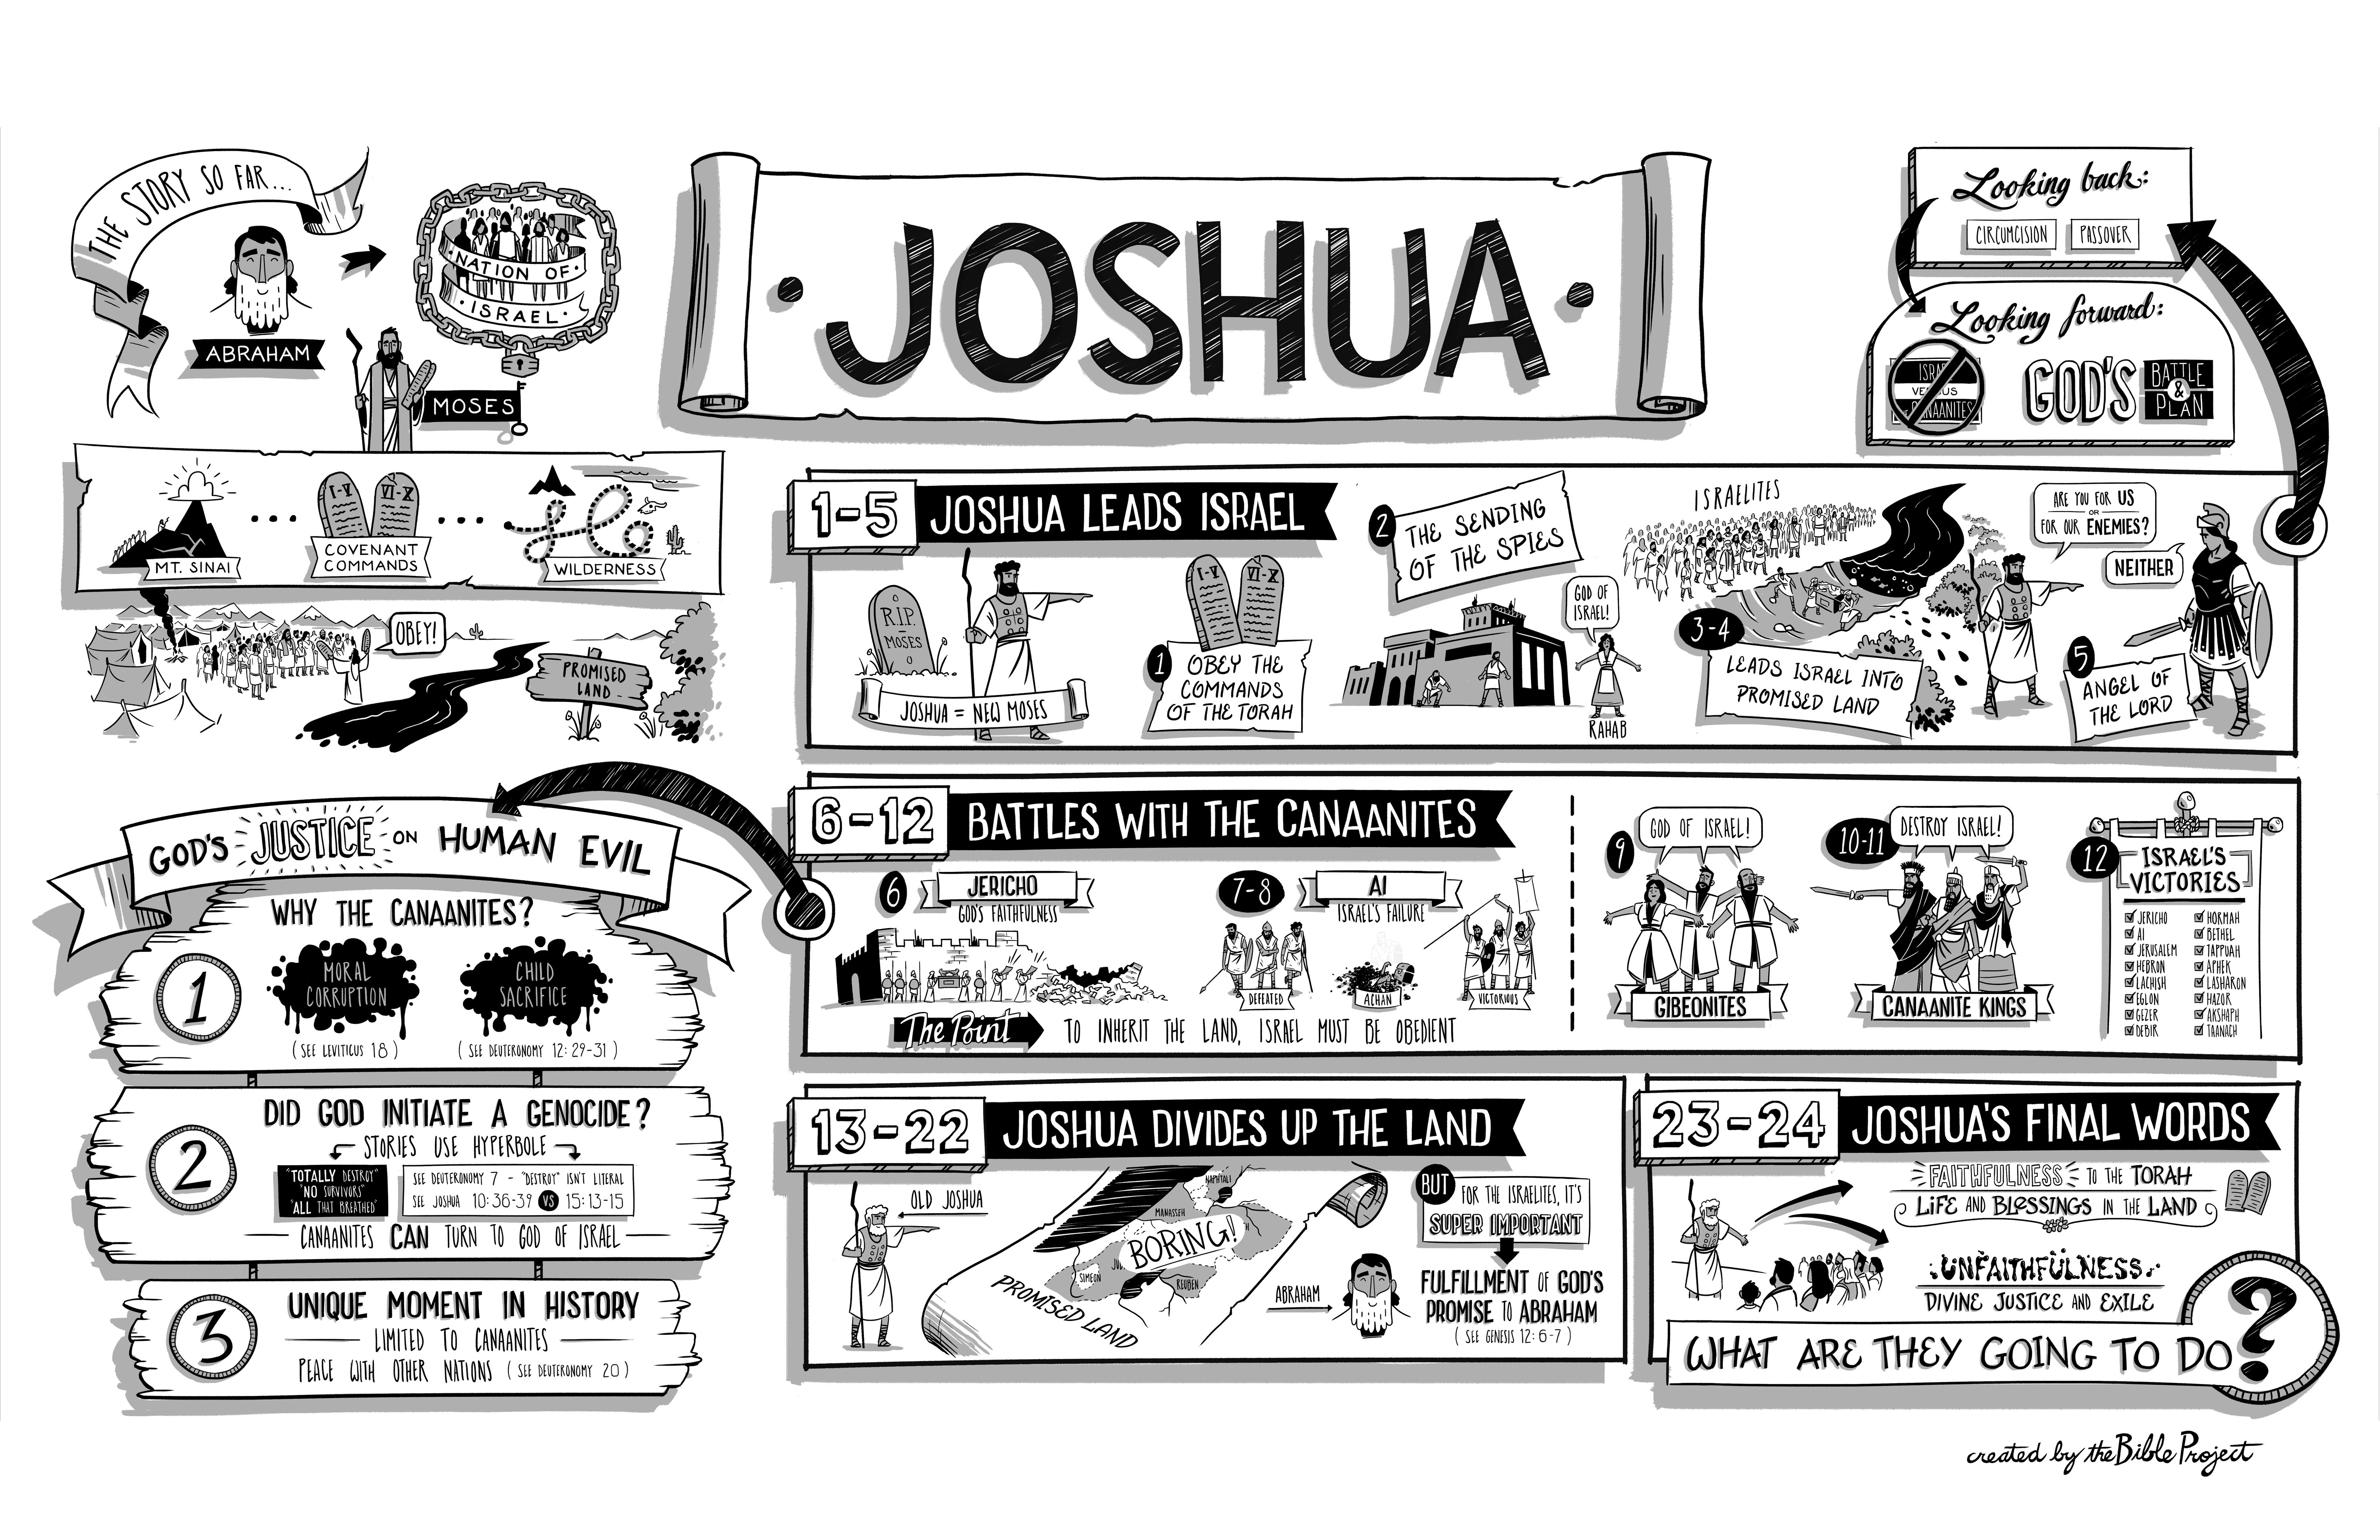
\includegraphics[scale=0.5, angle=90]{06OT-Joshua/References/1.BibleProject-Joshua.jpg}
\caption[Joshua from the Bible Project]{Joshua from the Bible Project}
\label{fig:Joshua from the Bible Project}
\end{center}
\end{figure}

\newpage
\begin{figure}
\begin{center}
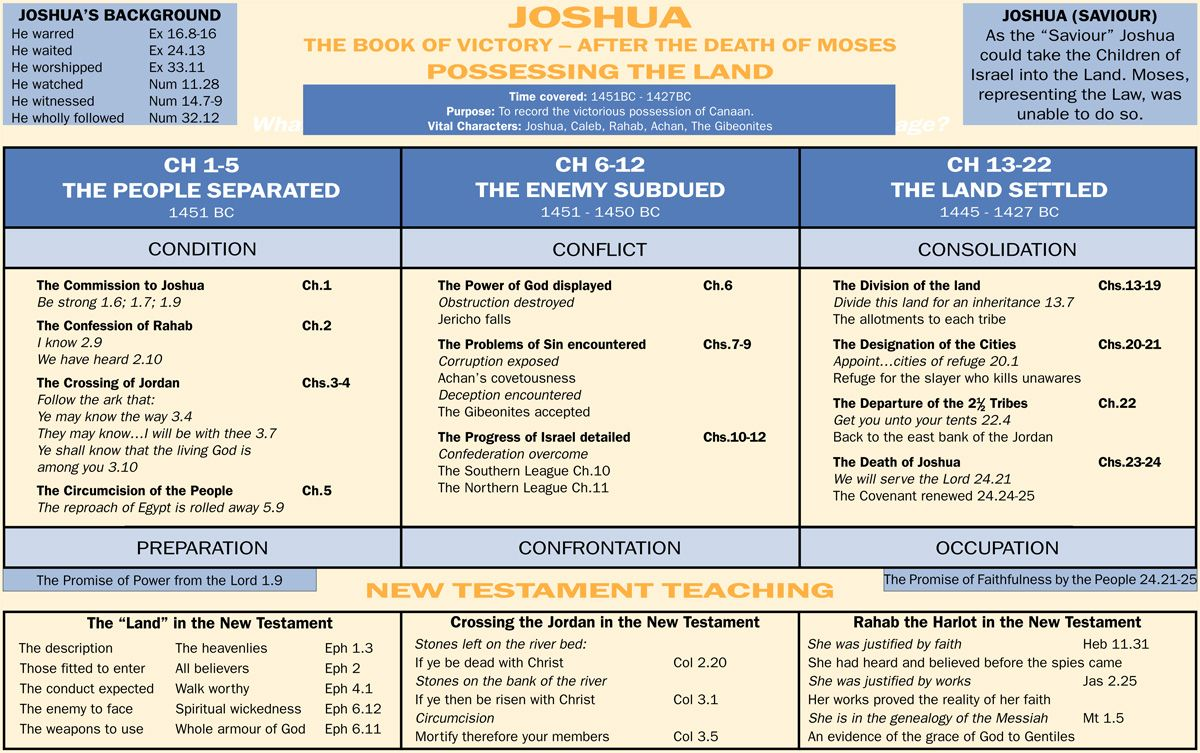
\includegraphics[scale=0.5, angle=90]{06OT-Joshua/References/2.JohnGrant-Joshua.jpg}
\caption[Joshua from John Grant]{Joshua from John Grant}
\label{fig:Joshua from John Grant}
\end{center}
\end{figure}

\newpage
\begin{figure}
\begin{center}
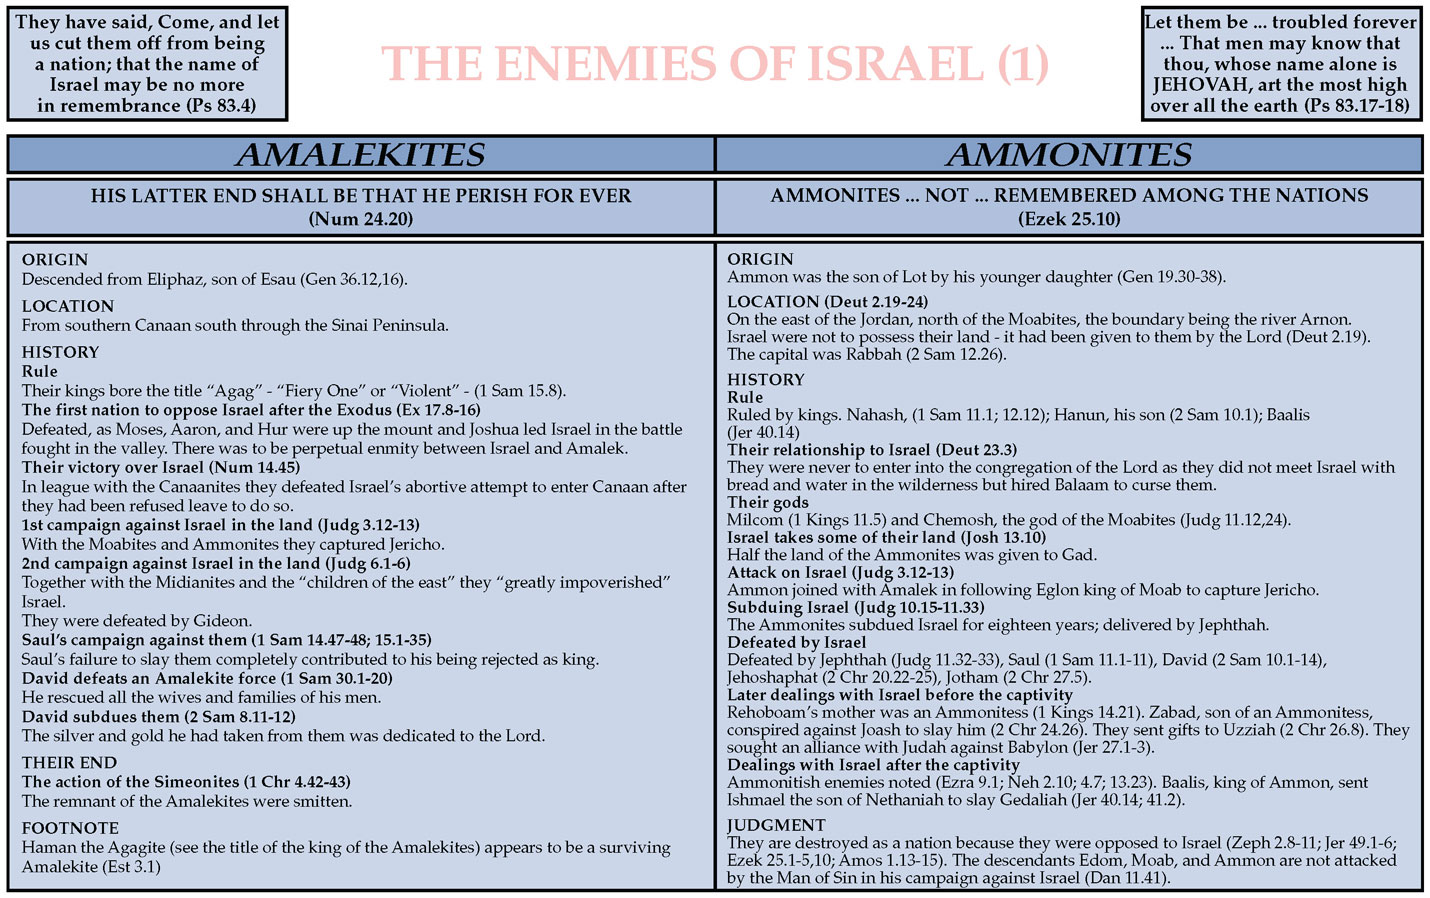
\includegraphics[scale=0.4, angle=90]{06OT-Joshua/References/3.EnemiesOfIsrael1.jpg}
\caption[Enemies of Israel 1]{Enemies of Israel 1}
\label{fig:Enemies of Israel 1}
\end{center}
\end{figure}

\newpage
\begin{figure}
\begin{center}
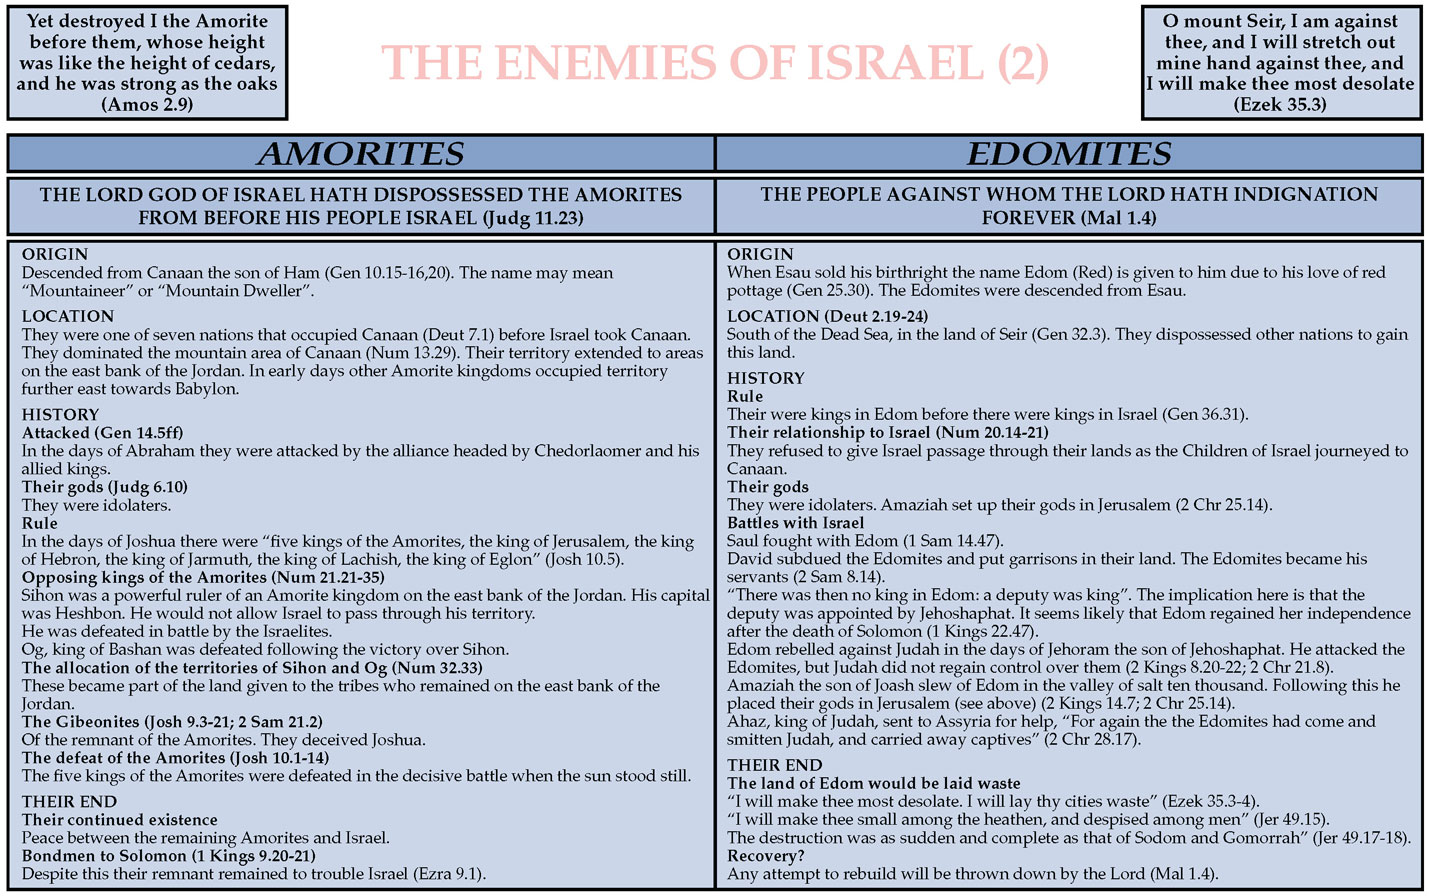
\includegraphics[scale=0.4, angle=90]{06OT-Joshua/References/4.EnemiesOfIsrael2.jpg}
\caption[Enemies of Israel 2]{Enemies of Israel 2}
\label{fig:Enemies of Israel 2}
\end{center}
\end{figure}

\newpage
\begin{figure}
\begin{center}
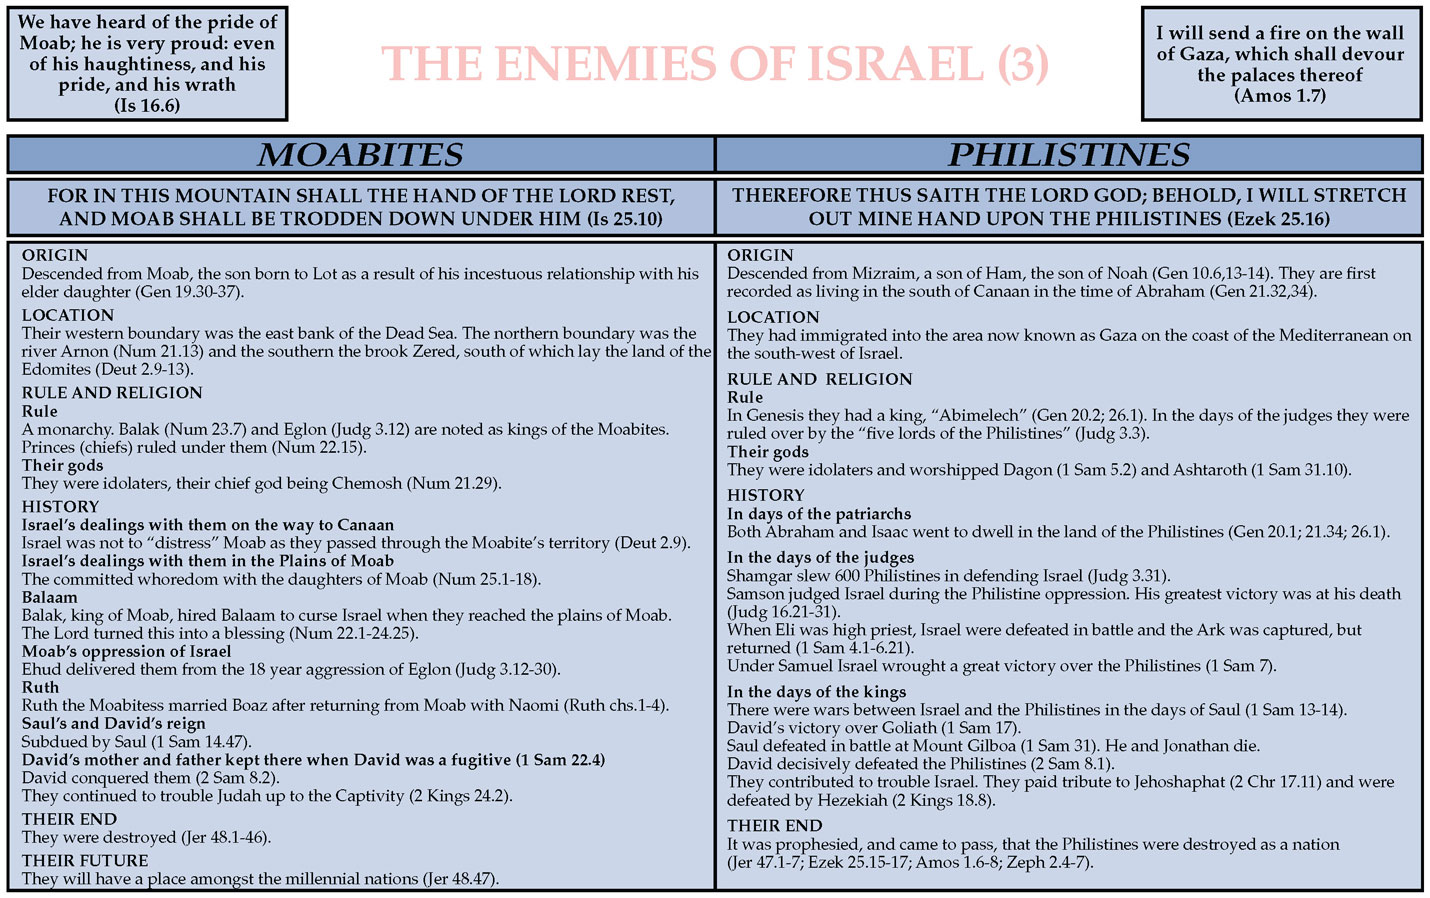
\includegraphics[scale=0.4, angle=90]{06OT-Joshua/References/5.EnemiesOfIsrael3.jpg}
\caption[Enemies of Israel 3]{Enemies of Israel 3}
\label{fig:Enemies of Israel 3}
\end{center}
\end{figure}

\newpage
\begin{figure}
\begin{center}
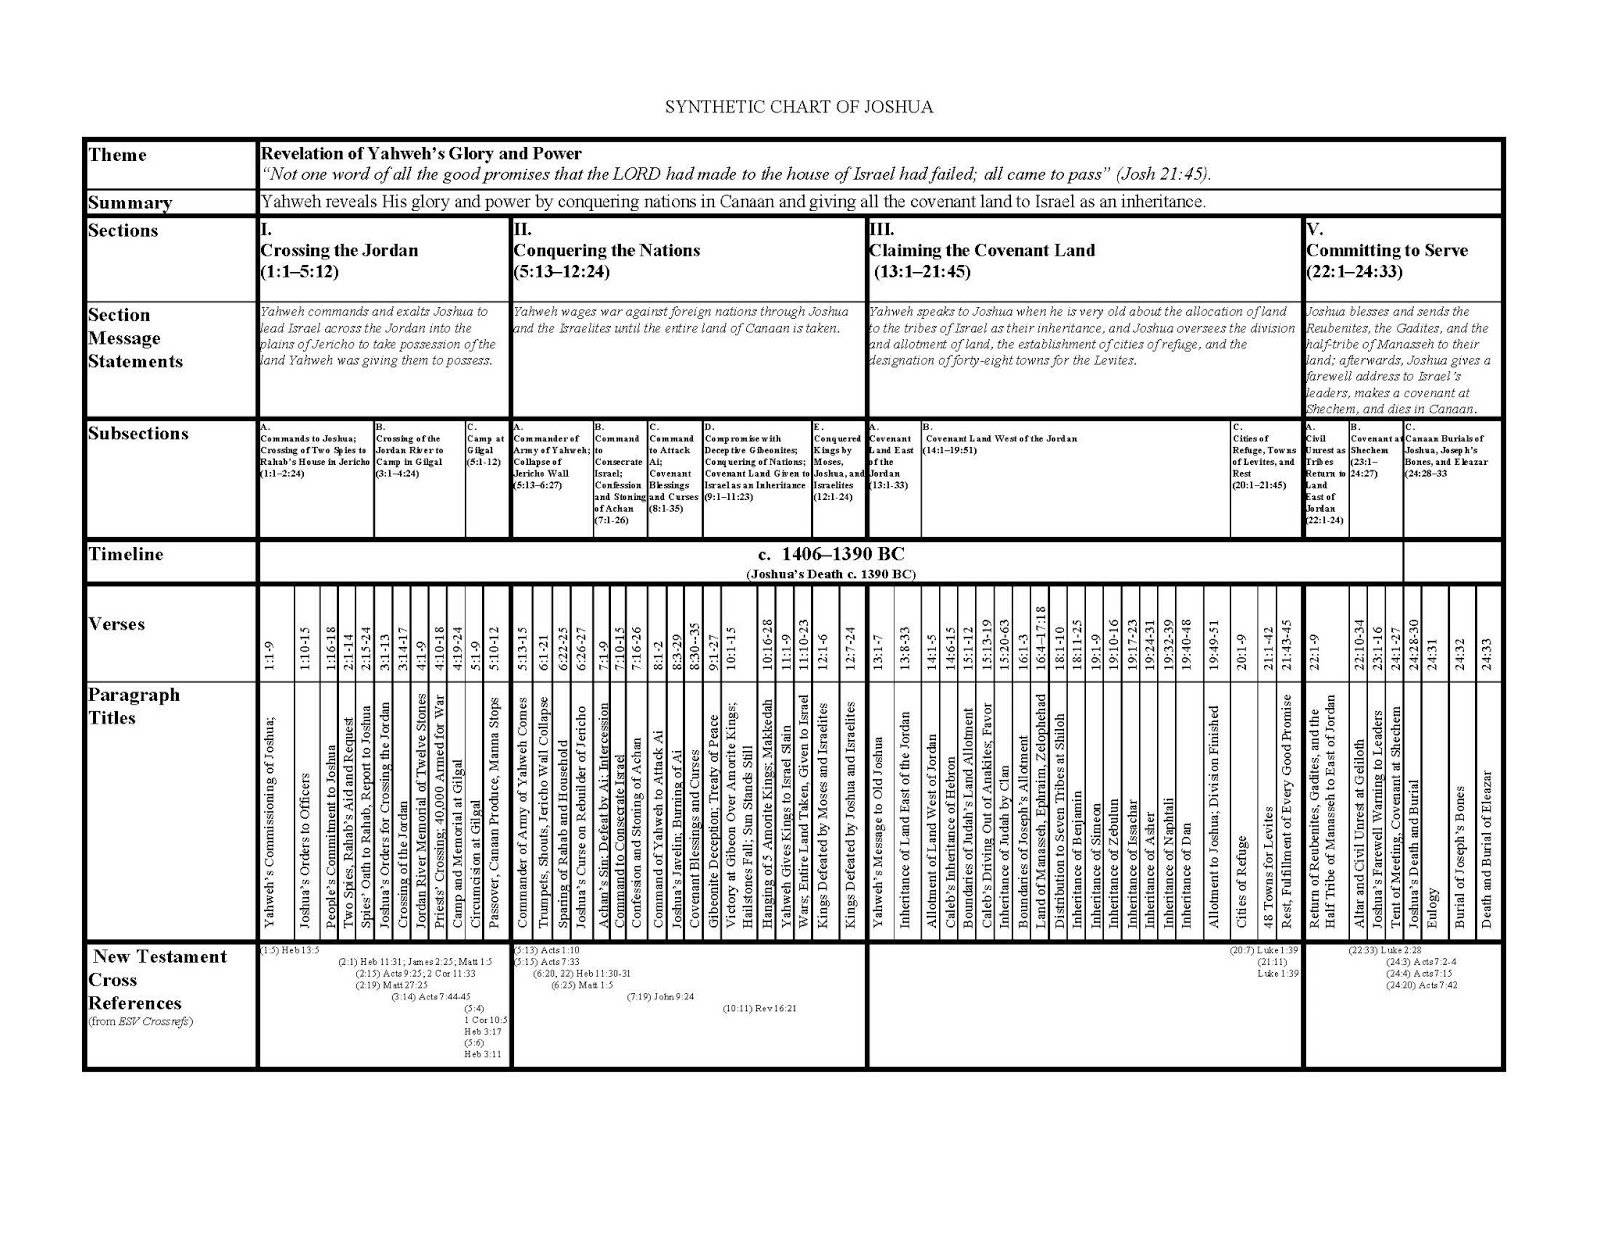
\includegraphics[scale=.4, angle=90]{06OT-Joshua/References/6.SyntheticChartofJoshua.jpg}
\caption[Synthetic Chart of Joshua]{Synthetic Chart of Joshua}
\label{fig:Synthetic Chart of Joshua}
\end{center}
\end{figure}


\newpage
\begin{figure}
\begin{center}
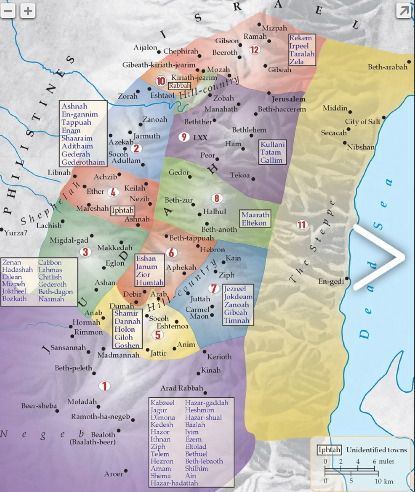
\includegraphics[scale=1, angle=0]{06OT-Joshua/References/7.WestSideOfDeadSea.jpg}
\caption[The West Side of the Dead Sea]{The West Side of the Dead Sea}
\label{fig:The West Side of the Dead Sea}
\end{center}
\end{figure}


\newpage
\begin{figure}
\begin{center}
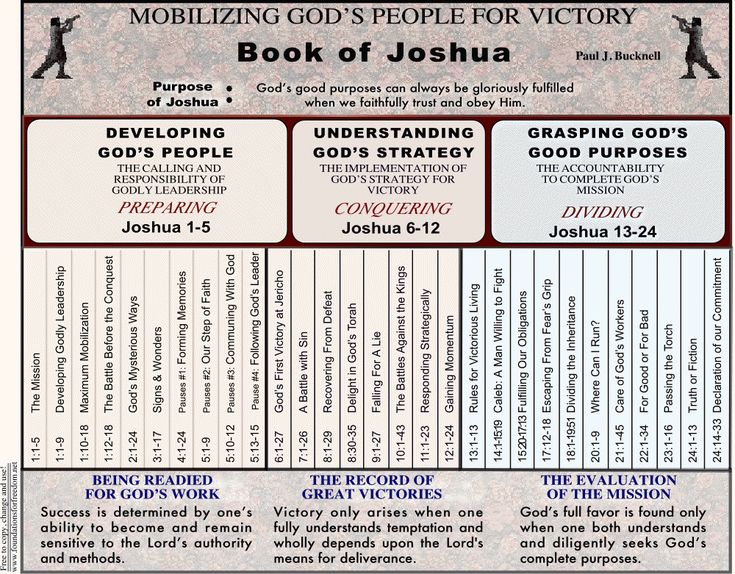
\includegraphics[scale=0.75, angle=90]{06OT-Joshua/References/8.Bucknell-Joshua.jpg}
\caption[Joshua from Bucknell]{Joshua from Bucknell}
\label{fig:Joshua from Bucknell}
\end{center}
\end{figure}


%\newpage
%\begin{figure}
%\begin{center}
%\includegraphics[scale=2, angle=90]{06OT-Joshua/References/9.Jensen-Joshua.png}
%\caption[Joshua from Jensen]{Joshua from Jensen}
%\label{fig:Joshua from Jensen}
%\end{center}
%\end{figure}


\newpage
\begin{figure}
\begin{center}
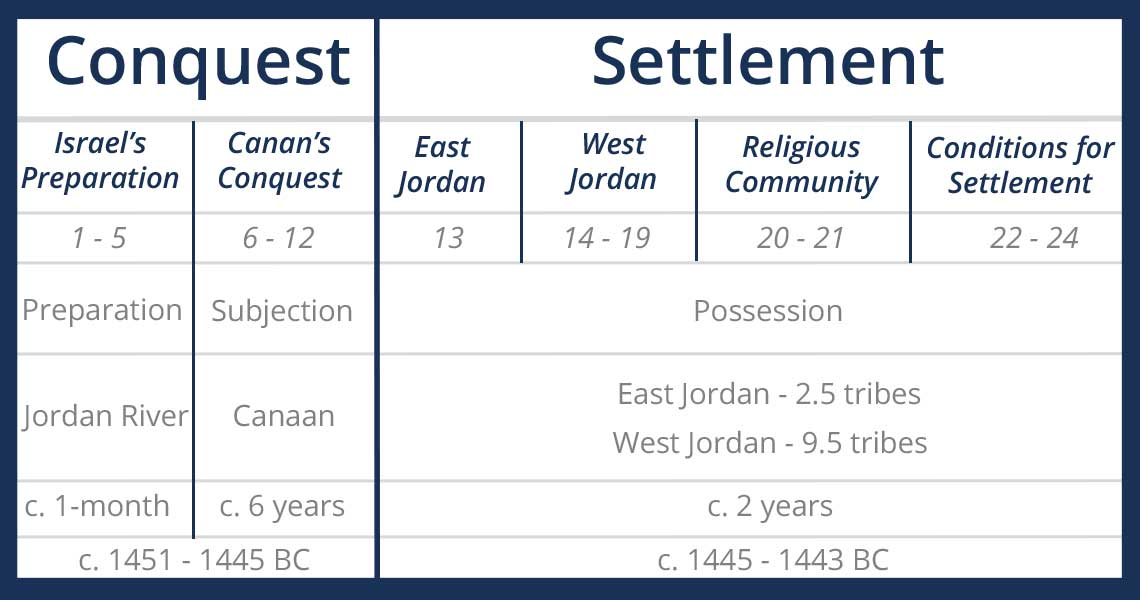
\includegraphics[scale=.5, angle=90]{06OT-Joshua/References/10.Bible-Brief-Joshua.jpg}
\caption[Bible Brief for Joshua]{Bible Brief for Joshua}
\label{fig:Bible Brief for Joshua}
\end{center}
\end{figure}

\newpage
\begin{figure}
\begin{center}
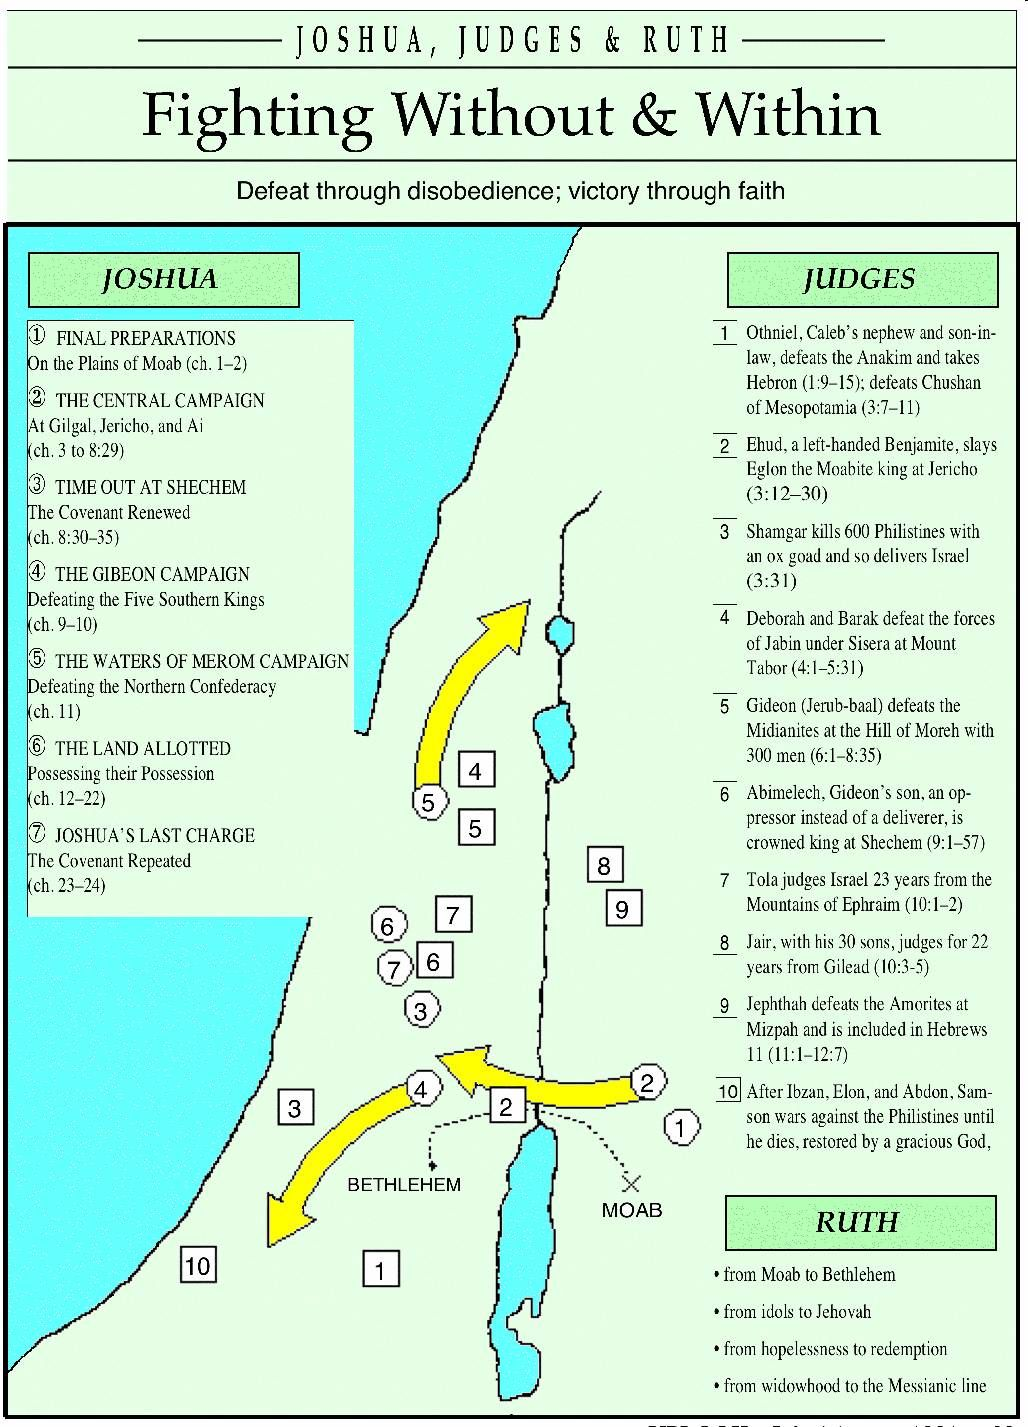
\includegraphics[scale=.5, angle=0]{06OT-Joshua/References/11.FightingInJoshuaAndJudges.jpg}
\caption[The Fighting in Joshua and Judges]{The Fighting in Joshua and Judges}
\label{fig:The Fighting in Joshua and Judges}
\end{center}
\end{figure}

\newpage
\begin{figure}
\begin{center}
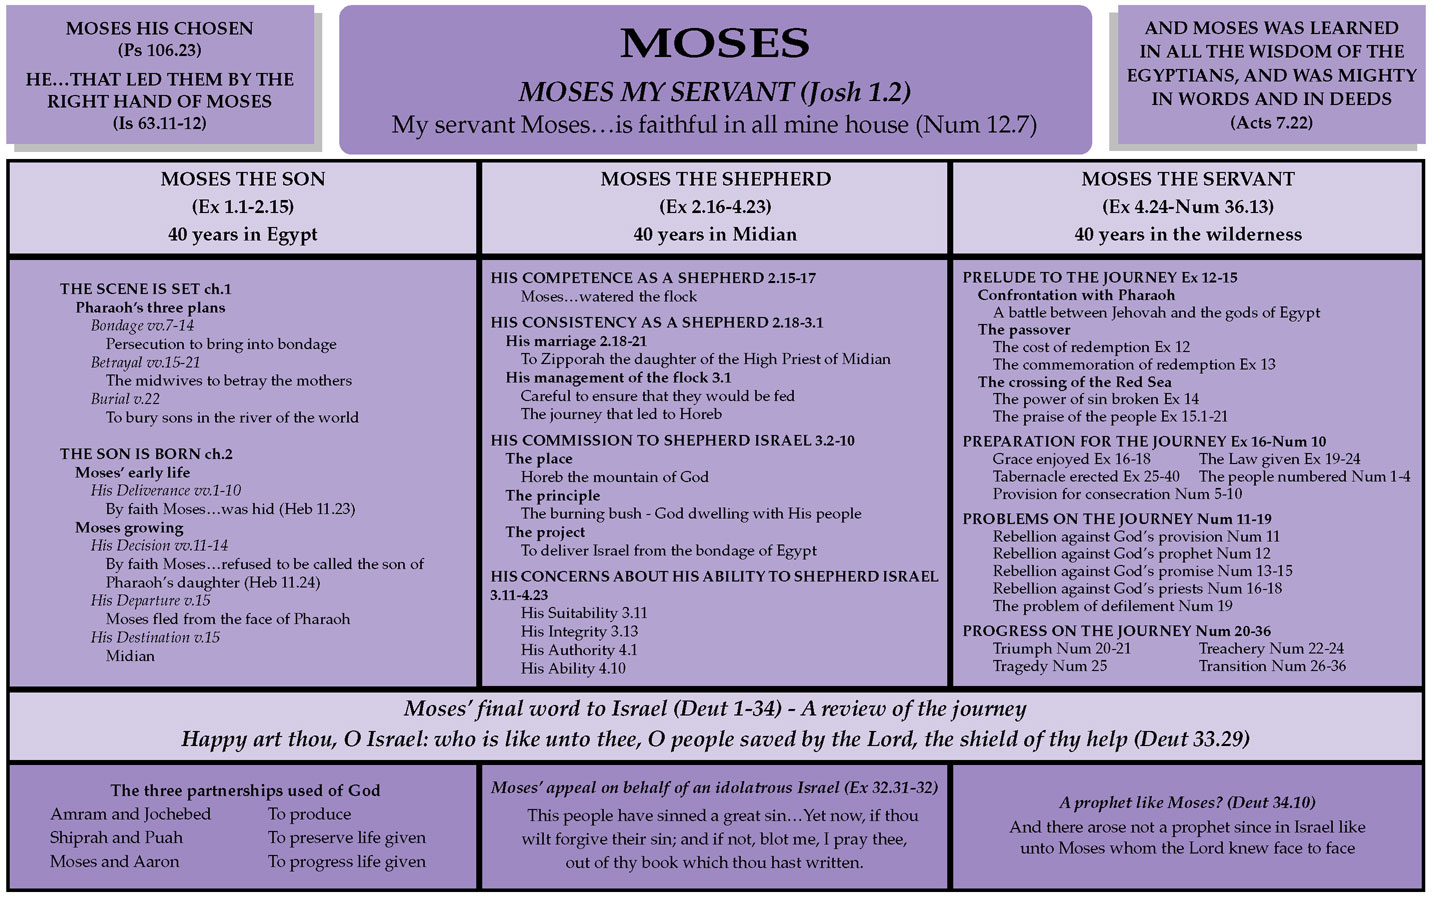
\includegraphics[scale=.4, angle=90]{06OT-Joshua/References/12.JohnGrantMoses.jpg}
\caption[Moses from John Grant]{Moses from John Grant}
\label{fig:Moses from John Grant}
\end{center}
\end{figure}







\chapter{Psalm 40}

\begin{figure}
  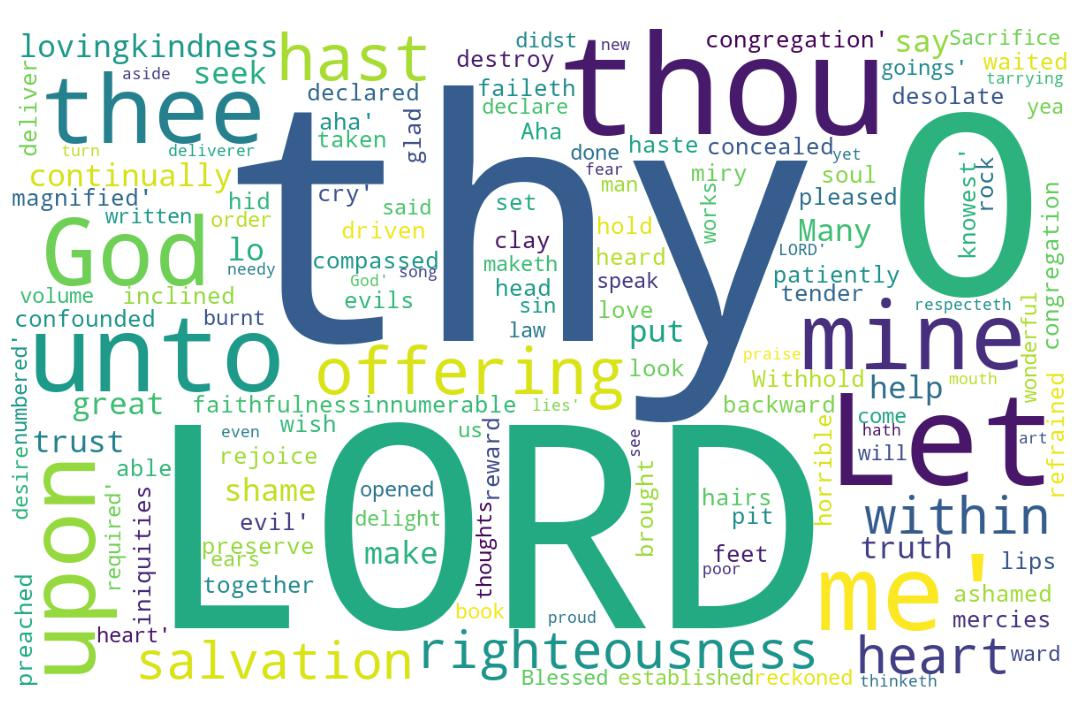
\includegraphics[width=\linewidth]{19OT-Psalms/Psalm40-WordCloud.jpg}
  \caption{Psalm 40 Word Cloud}
  \label{fig:Psalm 40 word Cloud}
\end{figure}

\marginpar{\scriptsize \centering \fcolorbox{bone}{lime}{\textbf{RESCUED}}\\ (Psalm 40:1-17) \begin{compactenum}[I.][8]
    \item \textbf{Patience} \index[scripture]{Psalms!Psa 040:01}(Psa 40:1)
    \item \textbf{Pit} \index[scripture]{Psalms!Psa 040:02}(Psa 40:2)
    \item \textbf{Praise} \index[scripture]{Psalms!Psa 040:03}(Psa 40:3)
    \item \textbf{Pride} to be avoided \index[scripture]{Psalms!Psa 040:04}(Psa 40:4)
   \item \textbf{Preaching} \index[scripture]{Psalms!Psa 040:09}(Psa 40:9)
    \item \textbf{Preservation} \index[scripture]{Psalms!Psa 040:11}(Psa 40:11)
    \item \textbf{Presence} of evil \index[scripture]{Psalms!Psa 040:12}(Psa 40:12)
\end{compactenum}}

\footnote{\textcolor[cmyk]{0.99998,1,0,0}{\hyperlink{TOC}{Return to end of Table of Contents.}}}\footnote{\href{https://audiobible.com/bible}{\textcolor[cmyk]{0.99998,1,0,0}{Psalms Audio}}}\textcolor[cmyk]{0.99998,1,0,0}{To the chief Musician, A Psalm of David.}\\
\\
\textcolor[cmyk]{0.99998,1,0,0}{I waited \fcolorbox{bone}{lime}{patiently} for the LORD; and he inclined unto \fcolorbox{bone}{bone}{me}, and heard my cry.}
[2] \textcolor[cmyk]{0.99998,1,0,0}{He brought \fcolorbox{bone}{bone}{me} up also out of an horrible \fcolorbox{bone}{lime}{pit}, out of the miry clay, and set my feet upon a rock, \emph{and} established my goings.}
[3] \textcolor[cmyk]{0.99998,1,0,0}{And he hath put a new song in my mouth, \emph{even} \fcolorbox{bone}{lime}{praise} unto our God: many shall see \emph{it}, and fear, and shall trust in the LORD.}
[4] \textcolor[cmyk]{0.99998,1,0,0}{Blessed \emph{is} that man that maketh the LORD his trust, and respecteth not the \fcolorbox{bone}{lime}{proud}, nor such as turn aside to lies.}
[5] \textcolor[cmyk]{0.99998,1,0,0}{Many, O LORD my God, \emph{are} \fcolorbox{bone}{bone}{thy} wonderful works \emph{which} thou hast done, and \fcolorbox{bone}{bone}{thy} thoughts \emph{which} \emph{are} to us-ward: they cannot be reckoned up in order unto thee: \emph{if} I would declare and speak \emph{of} \emph{them}, they are more than can be numbered.}
[6] \textcolor[cmyk]{0.99998,1,0,0}{Sacrifice and offering thou didst not desire; mine ears hast thou opened: burnt offering and sin offering hast thou not required.}
[7] \textcolor[cmyk]{0.99998,1,0,0}{Then said I, Lo, I come: in the volume of the book \emph{it} \emph{is} written of \fcolorbox{bone}{bone}{me},}
[8] \textcolor[cmyk]{0.99998,1,0,0}{I delight to do \fcolorbox{bone}{bone}{thy} will, O my God: yea, \fcolorbox{bone}{bone}{thy} law \emph{is} within my heart.}
[9] \textcolor[cmyk]{0.99998,1,0,0}{I have \fcolorbox{bone}{lime}{preached} righteousness in the great congregation: lo, I have not refrained my lips, O LORD, thou knowest.}
[10] \textcolor[cmyk]{0.99998,1,0,0}{I have not hid \fcolorbox{bone}{bone}{thy} righteousness within my heart; I have declared \fcolorbox{bone}{bone}{thy} faithfulness and \fcolorbox{bone}{bone}{thy} salvation: I have not concealed \fcolorbox{bone}{bone}{thy} lovingkindness and \fcolorbox{bone}{bone}{thy} truth from the great congregation.}
[11] \textcolor[cmyk]{0.99998,1,0,0}{Withhold not thou \fcolorbox{bone}{bone}{thy} tender mercies from \fcolorbox{bone}{bone}{me}, O LORD: let \fcolorbox{bone}{bone}{thy} lovingkindness and \fcolorbox{bone}{bone}{thy} truth continually \fcolorbox{bone}{lime}{preserve} \fcolorbox{bone}{bone}{me}.}
[12] \textcolor[cmyk]{0.99998,1,0,0}{For innumerable evils have \fcolorbox{bone}{lime}{compassed} \fcolorbox{bone}{bone}{me} about: mine iniquities have taken hold upon \fcolorbox{bone}{bone}{me}, so that I am not able to look up; they are more than the hairs of mine head: therefore my heart faileth \fcolorbox{bone}{bone}{me}.}
[13] \textcolor[cmyk]{0.99998,1,0,0}{Be pleased, O LORD, to deliver \fcolorbox{bone}{bone}{me}: O LORD, make haste to help \fcolorbox{bone}{bone}{me}.}
[14] \textcolor[cmyk]{0.99998,1,0,0}{Let them be ashamed and confounded together that seek after my soul to destroy it; let them be driven backward and put to shame that wish \fcolorbox{bone}{bone}{me} evil.}
[15] \textcolor[cmyk]{0.99998,1,0,0}{Let them be desolate for a reward of their shame that say unto \fcolorbox{bone}{bone}{me}, Aha, aha.}
[16] \textcolor[cmyk]{0.99998,1,0,0}{Let all those that seek thee rejoice and be glad in thee: let such as love \fcolorbox{bone}{bone}{thy} salvation say continually, The LORD be magnified.}
[17] \textcolor[cmyk]{0.99998,1,0,0}{But I \emph{am} poor and needy; \emph{yet} the Lord thinketh upon \fcolorbox{bone}{bone}{me}: thou \emph{art} my help and my deliverer; make no tarrying, O my God.}




\section{Psalm 40 Comments}

\subsection{Numeric Nuggets}
The words ``me'' and ``thy'' are found 13 times in the chapter. The 13-letter word ``righteousness'' is found in the chapter.

\subsection{Psalm 40:1}
The word ``inclined'' is one of those words found 13 times in scripture (Judges 9:3, Psalms 40:1, 116:2, 119:112, Proverbs 5:13, Jeremiah 7:24, 7:26, 11:8, 17:23, 25:4, 34:14, 35:15, and 44:5). 
%\index[NWIV]{15!Psalms!Psa 40:1}\index[AWIP]{I!Psalms!Psa 40:1}\index[AWIP]{waited!Psalms!Psa 40:1}\index[AWIP]{patiently!Psalms!Psa 40:1}\index[AWIP]{for!Psalms!Psa 40:1}\index[AWIP]{the!Psalms!Psa 40:1}\index[AWIP]{LORD!Psalms!Psa 40:1}\index[AWIP]{and!Psalms!Psa 40:1}\index[AWIP]{and!Psalms!Psa 40:1 (2)}\index[AWIP]{he!Psalms!Psa 40:1}\index[AWIP]{inclined!Psalms!Psa 40:1}\index[AWIP]{unto!Psalms!Psa 40:1}\index[AWIP]{me!Psalms!Psa 40:1}\index[AWIP]{heard!Psalms!Psa 40:1}\index[AWIP]{my!Psalms!Psa 40:1}\index[AWIP]{cry!Psalms!Psa 40:1}

\index[NWIV]{26!Psalms!Psa 40:2}\index[AWIP]{He!Psalms!Psa 40:2}\index[AWIP]{brought!Psalms!Psa 40:2}\index[AWIP]{me!Psalms!Psa 40:2}\index[AWIP]{up!Psalms!Psa 40:2}\index[AWIP]{also!Psalms!Psa 40:2}\index[AWIP]{out!Psalms!Psa 40:2}\index[AWIP]{out!Psalms!Psa 40:2 (2)}\index[AWIP]{of!Psalms!Psa 40:2}\index[AWIP]{of!Psalms!Psa 40:2 (2)}\index[AWIP]{an!Psalms!Psa 40:2}\index[AWIP]{horrible!Psalms!Psa 40:2}\index[AWIP]{pit!Psalms!Psa 40:2}\index[AWIP]{the!Psalms!Psa 40:2}\index[AWIP]{miry!Psalms!Psa 40:2}\index[AWIP]{clay!Psalms!Psa 40:2}\index[AWIP]{and!Psalms!Psa 40:2}\index[AWIP]{set!Psalms!Psa 40:2}\index[AWIP]{my!Psalms!Psa 40:2}\index[AWIP]{my!Psalms!Psa 40:2 (2)}\index[AWIP]{feet!Psalms!Psa 40:2}\index[AWIP]{upon!Psalms!Psa 40:2}\index[AWIP]{a!Psalms!Psa 40:2}\index[AWIP]{rock!Psalms!Psa 40:2}\index[AWIP]{\emph{and}!Psalms!Psa 40:2}\index[AWIP]{established!Psalms!Psa 40:2}\index[AWIP]{goings!Psalms!Psa 40:2}\index[AWIP]{\emph{and}!Psalms!Psa 40:2}

\index[NWIV]{27!Psalms!Psa 40:3}\index[AWIP]{And!Psalms!Psa 40:3}\index[AWIP]{he!Psalms!Psa 40:3}\index[AWIP]{hath!Psalms!Psa 40:3}\index[AWIP]{put!Psalms!Psa 40:3}\index[AWIP]{a!Psalms!Psa 40:3}\index[AWIP]{new!Psalms!Psa 40:3}\index[AWIP]{song!Psalms!Psa 40:3}\index[AWIP]{in!Psalms!Psa 40:3}\index[AWIP]{in!Psalms!Psa 40:3 (2)}\index[AWIP]{my!Psalms!Psa 40:3}\index[AWIP]{mouth!Psalms!Psa 40:3}\index[AWIP]{\emph{even}!Psalms!Psa 40:3}\index[AWIP]{praise!Psalms!Psa 40:3}\index[AWIP]{unto!Psalms!Psa 40:3}\index[AWIP]{our!Psalms!Psa 40:3}\index[AWIP]{God!Psalms!Psa 40:3}\index[AWIP]{many!Psalms!Psa 40:3}\index[AWIP]{shall!Psalms!Psa 40:3}\index[AWIP]{shall!Psalms!Psa 40:3 (2)}\index[AWIP]{see!Psalms!Psa 40:3}\index[AWIP]{\emph{it}!Psalms!Psa 40:3}\index[AWIP]{and!Psalms!Psa 40:3}\index[AWIP]{and!Psalms!Psa 40:3 (2)}\index[AWIP]{fear!Psalms!Psa 40:3}\index[AWIP]{trust!Psalms!Psa 40:3}\index[AWIP]{the!Psalms!Psa 40:3}\index[AWIP]{LORD!Psalms!Psa 40:3}\index[AWIP]{\emph{even}!Psalms!Psa 40:3}\index[AWIP]{\emph{it}!Psalms!Psa 40:3}

\index[NWIV]{22!Psalms!Psa 40:4}\index[AWIP]{Blessed!Psalms!Psa 40:4}\index[AWIP]{\emph{is}!Psalms!Psa 40:4}\index[AWIP]{that!Psalms!Psa 40:4}\index[AWIP]{that!Psalms!Psa 40:4 (2)}\index[AWIP]{man!Psalms!Psa 40:4}\index[AWIP]{maketh!Psalms!Psa 40:4}\index[AWIP]{the!Psalms!Psa 40:4}\index[AWIP]{the!Psalms!Psa 40:4 (2)}\index[AWIP]{LORD!Psalms!Psa 40:4}\index[AWIP]{his!Psalms!Psa 40:4}\index[AWIP]{trust!Psalms!Psa 40:4}\index[AWIP]{and!Psalms!Psa 40:4}\index[AWIP]{respecteth!Psalms!Psa 40:4}\index[AWIP]{not!Psalms!Psa 40:4}\index[AWIP]{proud!Psalms!Psa 40:4}\index[AWIP]{nor!Psalms!Psa 40:4}\index[AWIP]{such!Psalms!Psa 40:4}\index[AWIP]{as!Psalms!Psa 40:4}\index[AWIP]{turn!Psalms!Psa 40:4}\index[AWIP]{aside!Psalms!Psa 40:4}\index[AWIP]{to!Psalms!Psa 40:4}\index[AWIP]{lies!Psalms!Psa 40:4}\index[AWIP]{\emph{is}!Psalms!Psa 40:4}

\index[NWIV]{44!Psalms!Psa 40:5}\index[AWIP]{Many!Psalms!Psa 40:5}\index[AWIP]{O!Psalms!Psa 40:5}\index[AWIP]{LORD!Psalms!Psa 40:5}\index[AWIP]{my!Psalms!Psa 40:5}\index[AWIP]{God!Psalms!Psa 40:5}\index[AWIP]{\emph{are}!Psalms!Psa 40:5}\index[AWIP]{\emph{are}!Psalms!Psa 40:5 (2)}\index[AWIP]{thy!Psalms!Psa 40:5}\index[AWIP]{thy!Psalms!Psa 40:5 (2)}\index[AWIP]{wonderful!Psalms!Psa 40:5}\index[AWIP]{works!Psalms!Psa 40:5}\index[AWIP]{\emph{which}!Psalms!Psa 40:5}\index[AWIP]{\emph{which}!Psalms!Psa 40:5 (2)}\index[AWIP]{thou!Psalms!Psa 40:5}\index[AWIP]{hast!Psalms!Psa 40:5}\index[AWIP]{done!Psalms!Psa 40:5}\index[AWIP]{and!Psalms!Psa 40:5}\index[AWIP]{and!Psalms!Psa 40:5 (2)}\index[AWIP]{thoughts!Psalms!Psa 40:5}\index[AWIP]{to!Psalms!Psa 40:5}\index[AWIP]{us-ward!Psalms!Psa 40:5}\index[AWIP]{they!Psalms!Psa 40:5}\index[AWIP]{they!Psalms!Psa 40:5 (2)}\index[AWIP]{cannot!Psalms!Psa 40:5}\index[AWIP]{be!Psalms!Psa 40:5}\index[AWIP]{be!Psalms!Psa 40:5 (2)}\index[AWIP]{reckoned!Psalms!Psa 40:5}\index[AWIP]{up!Psalms!Psa 40:5}\index[AWIP]{in!Psalms!Psa 40:5}\index[AWIP]{order!Psalms!Psa 40:5}\index[AWIP]{unto!Psalms!Psa 40:5}\index[AWIP]{thee!Psalms!Psa 40:5}\index[AWIP]{\emph{if}!Psalms!Psa 40:5}\index[AWIP]{I!Psalms!Psa 40:5}\index[AWIP]{would!Psalms!Psa 40:5}\index[AWIP]{declare!Psalms!Psa 40:5}\index[AWIP]{speak!Psalms!Psa 40:5}\index[AWIP]{\emph{of}!Psalms!Psa 40:5}\index[AWIP]{\emph{them}!Psalms!Psa 40:5}\index[AWIP]{are!Psalms!Psa 40:5}\index[AWIP]{more!Psalms!Psa 40:5}\index[AWIP]{than!Psalms!Psa 40:5}\index[AWIP]{can!Psalms!Psa 40:5}\index[AWIP]{numbered!Psalms!Psa 40:5}\index[AWIP]{\emph{are}!Psalms!Psa 40:5}\index[AWIP]{\emph{are}!Psalms!Psa 40:5 (2)}\index[AWIP]{\emph{which}!Psalms!Psa 40:5}\index[AWIP]{\emph{which}!Psalms!Psa 40:5 (2)}\index[AWIP]{\emph{if}!Psalms!Psa 40:5}\index[AWIP]{\emph{of}!Psalms!Psa 40:5}\index[AWIP]{\emph{them}!Psalms!Psa 40:5}

\index[NWIV]{21!Psalms!Psa 40:6}\index[AWIP]{Sacrifice!Psalms!Psa 40:6}\index[AWIP]{and!Psalms!Psa 40:6}\index[AWIP]{and!Psalms!Psa 40:6 (2)}\index[AWIP]{offering!Psalms!Psa 40:6}\index[AWIP]{offering!Psalms!Psa 40:6 (2)}\index[AWIP]{offering!Psalms!Psa 40:6 (3)}\index[AWIP]{thou!Psalms!Psa 40:6}\index[AWIP]{thou!Psalms!Psa 40:6 (2)}\index[AWIP]{thou!Psalms!Psa 40:6 (3)}\index[AWIP]{didst!Psalms!Psa 40:6}\index[AWIP]{not!Psalms!Psa 40:6}\index[AWIP]{not!Psalms!Psa 40:6 (2)}\index[AWIP]{desire!Psalms!Psa 40:6}\index[AWIP]{mine!Psalms!Psa 40:6}\index[AWIP]{ears!Psalms!Psa 40:6}\index[AWIP]{hast!Psalms!Psa 40:6}\index[AWIP]{hast!Psalms!Psa 40:6 (2)}\index[AWIP]{opened!Psalms!Psa 40:6}\index[AWIP]{burnt!Psalms!Psa 40:6}\index[AWIP]{sin!Psalms!Psa 40:6}\index[AWIP]{required!Psalms!Psa 40:6}

\index[NWIV]{17!Psalms!Psa 40:7}\index[AWIP]{Then!Psalms!Psa 40:7}\index[AWIP]{said!Psalms!Psa 40:7}\index[AWIP]{I!Psalms!Psa 40:7}\index[AWIP]{I!Psalms!Psa 40:7 (2)}\index[AWIP]{Lo!Psalms!Psa 40:7}\index[AWIP]{come!Psalms!Psa 40:7}\index[AWIP]{in!Psalms!Psa 40:7}\index[AWIP]{the!Psalms!Psa 40:7}\index[AWIP]{the!Psalms!Psa 40:7 (2)}\index[AWIP]{volume!Psalms!Psa 40:7}\index[AWIP]{of!Psalms!Psa 40:7}\index[AWIP]{of!Psalms!Psa 40:7 (2)}\index[AWIP]{book!Psalms!Psa 40:7}\index[AWIP]{\emph{it}!Psalms!Psa 40:7}\index[AWIP]{\emph{is}!Psalms!Psa 40:7}\index[AWIP]{written!Psalms!Psa 40:7}\index[AWIP]{me!Psalms!Psa 40:7}\index[AWIP]{\emph{it}!Psalms!Psa 40:7}\index[AWIP]{\emph{is}!Psalms!Psa 40:7}

\index[NWIV]{16!Psalms!Psa 40:8}\index[AWIP]{I!Psalms!Psa 40:8}\index[AWIP]{delight!Psalms!Psa 40:8}\index[AWIP]{to!Psalms!Psa 40:8}\index[AWIP]{do!Psalms!Psa 40:8}\index[AWIP]{thy!Psalms!Psa 40:8}\index[AWIP]{thy!Psalms!Psa 40:8 (2)}\index[AWIP]{will!Psalms!Psa 40:8}\index[AWIP]{O!Psalms!Psa 40:8}\index[AWIP]{my!Psalms!Psa 40:8}\index[AWIP]{my!Psalms!Psa 40:8 (2)}\index[AWIP]{God!Psalms!Psa 40:8}\index[AWIP]{yea!Psalms!Psa 40:8}\index[AWIP]{law!Psalms!Psa 40:8}\index[AWIP]{\emph{is}!Psalms!Psa 40:8}\index[AWIP]{within!Psalms!Psa 40:8}\index[AWIP]{heart!Psalms!Psa 40:8}\index[AWIP]{\emph{is}!Psalms!Psa 40:8}

\index[NWIV]{19!Psalms!Psa 40:9}\index[AWIP]{I!Psalms!Psa 40:9}\index[AWIP]{I!Psalms!Psa 40:9 (2)}\index[AWIP]{have!Psalms!Psa 40:9}\index[AWIP]{have!Psalms!Psa 40:9 (2)}\index[AWIP]{preached!Psalms!Psa 40:9}\index[AWIP]{righteousness!Psalms!Psa 40:9}\index[AWIP]{in!Psalms!Psa 40:9}\index[AWIP]{the!Psalms!Psa 40:9}\index[AWIP]{great!Psalms!Psa 40:9}\index[AWIP]{congregation!Psalms!Psa 40:9}\index[AWIP]{lo!Psalms!Psa 40:9}\index[AWIP]{not!Psalms!Psa 40:9}\index[AWIP]{refrained!Psalms!Psa 40:9}\index[AWIP]{my!Psalms!Psa 40:9}\index[AWIP]{lips!Psalms!Psa 40:9}\index[AWIP]{O!Psalms!Psa 40:9}\index[AWIP]{LORD!Psalms!Psa 40:9}\index[AWIP]{thou!Psalms!Psa 40:9}\index[AWIP]{knowest!Psalms!Psa 40:9}

\index[NWIV]{30!Psalms!Psa 40:10}\index[AWIP]{I!Psalms!Psa 40:10}\index[AWIP]{I!Psalms!Psa 40:10 (2)}\index[AWIP]{I!Psalms!Psa 40:10 (3)}\index[AWIP]{have!Psalms!Psa 40:10}\index[AWIP]{have!Psalms!Psa 40:10 (2)}\index[AWIP]{have!Psalms!Psa 40:10 (3)}\index[AWIP]{not!Psalms!Psa 40:10}\index[AWIP]{not!Psalms!Psa 40:10 (2)}\index[AWIP]{hid!Psalms!Psa 40:10}\index[AWIP]{thy!Psalms!Psa 40:10}\index[AWIP]{thy!Psalms!Psa 40:10 (2)}\index[AWIP]{thy!Psalms!Psa 40:10 (3)}\index[AWIP]{thy!Psalms!Psa 40:10 (4)}\index[AWIP]{thy!Psalms!Psa 40:10 (5)}\index[AWIP]{righteousness!Psalms!Psa 40:10}\index[AWIP]{within!Psalms!Psa 40:10}\index[AWIP]{my!Psalms!Psa 40:10}\index[AWIP]{heart!Psalms!Psa 40:10}\index[AWIP]{declared!Psalms!Psa 40:10}\index[AWIP]{faithfulness!Psalms!Psa 40:10}\index[AWIP]{and!Psalms!Psa 40:10}\index[AWIP]{and!Psalms!Psa 40:10 (2)}\index[AWIP]{salvation!Psalms!Psa 40:10}\index[AWIP]{concealed!Psalms!Psa 40:10}\index[AWIP]{lovingkindness!Psalms!Psa 40:10}\index[AWIP]{truth!Psalms!Psa 40:10}\index[AWIP]{from!Psalms!Psa 40:10}\index[AWIP]{the!Psalms!Psa 40:10}\index[AWIP]{great!Psalms!Psa 40:10}\index[AWIP]{congregation!Psalms!Psa 40:10}

\index[NWIV]{19!Psalms!Psa 40:11}\index[AWIP]{Withhold!Psalms!Psa 40:11}\index[AWIP]{not!Psalms!Psa 40:11}\index[AWIP]{thou!Psalms!Psa 40:11}\index[AWIP]{thy!Psalms!Psa 40:11}\index[AWIP]{thy!Psalms!Psa 40:11 (2)}\index[AWIP]{thy!Psalms!Psa 40:11 (3)}\index[AWIP]{tender!Psalms!Psa 40:11}\index[AWIP]{mercies!Psalms!Psa 40:11}\index[AWIP]{from!Psalms!Psa 40:11}\index[AWIP]{me!Psalms!Psa 40:11}\index[AWIP]{me!Psalms!Psa 40:11 (2)}\index[AWIP]{O!Psalms!Psa 40:11}\index[AWIP]{LORD!Psalms!Psa 40:11}\index[AWIP]{let!Psalms!Psa 40:11}\index[AWIP]{lovingkindness!Psalms!Psa 40:11}\index[AWIP]{and!Psalms!Psa 40:11}\index[AWIP]{truth!Psalms!Psa 40:11}\index[AWIP]{continually!Psalms!Psa 40:11}\index[AWIP]{preserve!Psalms!Psa 40:11}

\index[NWIV]{37!Psalms!Psa 40:12}\index[AWIP]{For!Psalms!Psa 40:12}\index[AWIP]{innumerable!Psalms!Psa 40:12}\index[AWIP]{evils!Psalms!Psa 40:12}\index[AWIP]{have!Psalms!Psa 40:12}\index[AWIP]{have!Psalms!Psa 40:12 (2)}\index[AWIP]{compassed!Psalms!Psa 40:12}\index[AWIP]{me!Psalms!Psa 40:12}\index[AWIP]{me!Psalms!Psa 40:12 (2)}\index[AWIP]{me!Psalms!Psa 40:12 (3)}\index[AWIP]{about!Psalms!Psa 40:12}\index[AWIP]{mine!Psalms!Psa 40:12}\index[AWIP]{mine!Psalms!Psa 40:12 (2)}\index[AWIP]{iniquities!Psalms!Psa 40:12}\index[AWIP]{taken!Psalms!Psa 40:12}\index[AWIP]{hold!Psalms!Psa 40:12}\index[AWIP]{upon!Psalms!Psa 40:12}\index[AWIP]{so!Psalms!Psa 40:12}\index[AWIP]{that!Psalms!Psa 40:12}\index[AWIP]{I!Psalms!Psa 40:12}\index[AWIP]{am!Psalms!Psa 40:12}\index[AWIP]{not!Psalms!Psa 40:12}\index[AWIP]{able!Psalms!Psa 40:12}\index[AWIP]{to!Psalms!Psa 40:12}\index[AWIP]{look!Psalms!Psa 40:12}\index[AWIP]{up!Psalms!Psa 40:12}\index[AWIP]{they!Psalms!Psa 40:12}\index[AWIP]{are!Psalms!Psa 40:12}\index[AWIP]{more!Psalms!Psa 40:12}\index[AWIP]{than!Psalms!Psa 40:12}\index[AWIP]{the!Psalms!Psa 40:12}\index[AWIP]{hairs!Psalms!Psa 40:12}\index[AWIP]{of!Psalms!Psa 40:12}\index[AWIP]{head!Psalms!Psa 40:12}\index[AWIP]{therefore!Psalms!Psa 40:12}\index[AWIP]{my!Psalms!Psa 40:12}\index[AWIP]{heart!Psalms!Psa 40:12}\index[AWIP]{faileth!Psalms!Psa 40:12}

\index[NWIV]{14!Psalms!Psa 40:13}\index[AWIP]{Be!Psalms!Psa 40:13}\index[AWIP]{pleased!Psalms!Psa 40:13}\index[AWIP]{O!Psalms!Psa 40:13}\index[AWIP]{O!Psalms!Psa 40:13 (2)}\index[AWIP]{LORD!Psalms!Psa 40:13}\index[AWIP]{LORD!Psalms!Psa 40:13 (2)}\index[AWIP]{to!Psalms!Psa 40:13}\index[AWIP]{to!Psalms!Psa 40:13 (2)}\index[AWIP]{deliver!Psalms!Psa 40:13}\index[AWIP]{me!Psalms!Psa 40:13}\index[AWIP]{me!Psalms!Psa 40:13 (2)}\index[AWIP]{make!Psalms!Psa 40:13}\index[AWIP]{haste!Psalms!Psa 40:13}\index[AWIP]{help!Psalms!Psa 40:13}

\index[NWIV]{28!Psalms!Psa 40:14}\index[AWIP]{Let!Psalms!Psa 40:14}\index[AWIP]{them!Psalms!Psa 40:14}\index[AWIP]{them!Psalms!Psa 40:14 (2)}\index[AWIP]{be!Psalms!Psa 40:14}\index[AWIP]{be!Psalms!Psa 40:14 (2)}\index[AWIP]{ashamed!Psalms!Psa 40:14}\index[AWIP]{and!Psalms!Psa 40:14}\index[AWIP]{and!Psalms!Psa 40:14 (2)}\index[AWIP]{confounded!Psalms!Psa 40:14}\index[AWIP]{together!Psalms!Psa 40:14}\index[AWIP]{that!Psalms!Psa 40:14}\index[AWIP]{that!Psalms!Psa 40:14 (2)}\index[AWIP]{seek!Psalms!Psa 40:14}\index[AWIP]{after!Psalms!Psa 40:14}\index[AWIP]{my!Psalms!Psa 40:14}\index[AWIP]{soul!Psalms!Psa 40:14}\index[AWIP]{to!Psalms!Psa 40:14}\index[AWIP]{to!Psalms!Psa 40:14 (2)}\index[AWIP]{destroy!Psalms!Psa 40:14}\index[AWIP]{it!Psalms!Psa 40:14}\index[AWIP]{let!Psalms!Psa 40:14}\index[AWIP]{driven!Psalms!Psa 40:14}\index[AWIP]{backward!Psalms!Psa 40:14}\index[AWIP]{put!Psalms!Psa 40:14}\index[AWIP]{shame!Psalms!Psa 40:14}\index[AWIP]{wish!Psalms!Psa 40:14}\index[AWIP]{me!Psalms!Psa 40:14}\index[AWIP]{evil!Psalms!Psa 40:14}

\index[NWIV]{16!Psalms!Psa 40:15}\index[AWIP]{Let!Psalms!Psa 40:15}\index[AWIP]{them!Psalms!Psa 40:15}\index[AWIP]{be!Psalms!Psa 40:15}\index[AWIP]{desolate!Psalms!Psa 40:15}\index[AWIP]{for!Psalms!Psa 40:15}\index[AWIP]{a!Psalms!Psa 40:15}\index[AWIP]{reward!Psalms!Psa 40:15}\index[AWIP]{of!Psalms!Psa 40:15}\index[AWIP]{their!Psalms!Psa 40:15}\index[AWIP]{shame!Psalms!Psa 40:15}\index[AWIP]{that!Psalms!Psa 40:15}\index[AWIP]{say!Psalms!Psa 40:15}\index[AWIP]{unto!Psalms!Psa 40:15}\index[AWIP]{me!Psalms!Psa 40:15}\index[AWIP]{Aha!Psalms!Psa 40:15}\index[AWIP]{aha!Psalms!Psa 40:15}

\index[NWIV]{24!Psalms!Psa 40:16}\index[AWIP]{Let!Psalms!Psa 40:16}\index[AWIP]{all!Psalms!Psa 40:16}\index[AWIP]{those!Psalms!Psa 40:16}\index[AWIP]{that!Psalms!Psa 40:16}\index[AWIP]{seek!Psalms!Psa 40:16}\index[AWIP]{thee!Psalms!Psa 40:16}\index[AWIP]{thee!Psalms!Psa 40:16 (2)}\index[AWIP]{rejoice!Psalms!Psa 40:16}\index[AWIP]{and!Psalms!Psa 40:16}\index[AWIP]{be!Psalms!Psa 40:16}\index[AWIP]{be!Psalms!Psa 40:16 (2)}\index[AWIP]{glad!Psalms!Psa 40:16}\index[AWIP]{in!Psalms!Psa 40:16}\index[AWIP]{let!Psalms!Psa 40:16}\index[AWIP]{such!Psalms!Psa 40:16}\index[AWIP]{as!Psalms!Psa 40:16}\index[AWIP]{love!Psalms!Psa 40:16}\index[AWIP]{thy!Psalms!Psa 40:16}\index[AWIP]{salvation!Psalms!Psa 40:16}\index[AWIP]{say!Psalms!Psa 40:16}\index[AWIP]{continually!Psalms!Psa 40:16}\index[AWIP]{The!Psalms!Psa 40:16}\index[AWIP]{LORD!Psalms!Psa 40:16}\index[AWIP]{magnified!Psalms!Psa 40:16}

\index[NWIV]{25!Psalms!Psa 40:17}\index[AWIP]{But!Psalms!Psa 40:17}\index[AWIP]{I!Psalms!Psa 40:17}\index[AWIP]{\emph{am}!Psalms!Psa 40:17}\index[AWIP]{poor!Psalms!Psa 40:17}\index[AWIP]{and!Psalms!Psa 40:17}\index[AWIP]{and!Psalms!Psa 40:17 (2)}\index[AWIP]{needy!Psalms!Psa 40:17}\index[AWIP]{\emph{yet}!Psalms!Psa 40:17}\index[AWIP]{the!Psalms!Psa 40:17}\index[AWIP]{Lord!Psalms!Psa 40:17}\index[AWIP]{thinketh!Psalms!Psa 40:17}\index[AWIP]{upon!Psalms!Psa 40:17}\index[AWIP]{me!Psalms!Psa 40:17}\index[AWIP]{thou!Psalms!Psa 40:17}\index[AWIP]{\emph{art}!Psalms!Psa 40:17}\index[AWIP]{my!Psalms!Psa 40:17}\index[AWIP]{my!Psalms!Psa 40:17 (2)}\index[AWIP]{my!Psalms!Psa 40:17 (3)}\index[AWIP]{help!Psalms!Psa 40:17}\index[AWIP]{deliverer!Psalms!Psa 40:17}\index[AWIP]{make!Psalms!Psa 40:17}\index[AWIP]{no!Psalms!Psa 40:17}\index[AWIP]{tarrying!Psalms!Psa 40:17}\index[AWIP]{O!Psalms!Psa 40:17}\index[AWIP]{God!Psalms!Psa 40:17}\index[AWIP]{\emph{am}!Psalms!Psa 40:17}\index[AWIP]{\emph{yet}!Psalms!Psa 40:17}\index[AWIP]{\emph{art}!Psalms!Psa 40:17}


\section{Psalm 40 Outlines}

\subsection{My Outlines}

\subsubsection{Rescued}
%Psalm 40:\footnote{unknown, Keith Anthony}
\index[speaker]{Keith Anthony!Psalm 040 (Rescued)}
\index[series]{Psalms (Keith Anthony)!Psalm 040 (Rescued)}
\index[date]{2016/12/18!Psalm 040 (Rescued) (Keith Anthony)}
\begin{compactenum}[I.]
    \item \textbf{Patience} \index[scripture]{Psalms!Psa 040:01}(Psa 40:1)
    \item \textbf{Pit} \index[scripture]{Psalms!Psa 040:02}(Psa 40:2)
    \item \textbf{Praise} \index[scripture]{Psalms!Psa 040:03}(Psa 40:3)
    \item \textbf{Pride} to be avoided \index[scripture]{Psalms!Psa 040:04}(Psa 40:4)
   \item \textbf{Preaching} \index[scripture]{Psalms!Psa 040:09}(Psa 40:9)
    \item \textbf{Preservation} \index[scripture]{Psalms!Psa 040:11}(Psa 40:11)
    \item \textbf{Presence} of evil \index[scripture]{Psalms!Psa 040:12}(Psa 40:12)
\end{compactenum}


\subsection{Outlines from Others}

\subsubsection{Principles Pertaining To The Pit}
\index[speaker]{Michael Lovett!Psalm 040 (Principles Pertaining To The Pit)}
\index[series]{Psalms (Michael Lovett)!Psalm 040 (Principles Pertaining To The Pit)}
\index[date]{2014/1103!Psalm 040 (Principles Pertaining To The Pit) (Michael Lovett)}
Probably one of the Psalms  quoted frequently when preaching would be the one we have before us this morning. It is one of many passages that I truly cherish. It is and was such a blessing to me when I first came across it. I realized in many aspects that the truth contained within that verse was in many aspects what God did for me. You have heard me mention on more than one occasion that God picked me up out of an horrible pit, and He placed my feet upon a rock and He has established my goings…… and I say Thank you and Praise the Lord He did.

If you are not careful in life many times we can find ourselves in a place we would much rather not be. Most folks never intend for it to happen, but it does. They want to be in a better place, but many times “the Want To” gets overshadowed by “the Will To” and that is usually a result of a particular place that we have settled into. We call that place in today’s vernacular “a rut” however the Bible refers to it many times as a “pit.” For some they have either chosen to stay in their Pit or drag their Pit around with them and relish in the fact they have one.

As a Pastor I have come to realize that way too many folks live most of their life in a Pit. God never intended for us to reside in a Pit and if He so chooses for you to be in one, for a season (Joseph, Jeremiah) then He will inform you of the reason why, and the duration.

In my few years in this world I have come to realize that Pits come in all shapes and sizes. I have as well realized that there is no discrimination from the Pit, as to its inhabitants….it welcomes all dwellers. As I reflect in my mind in the Scriptures I find that many good folk as well as bad have spent time in “the Pit”. Some grow use to it while others long for and desire to get out of it. I want to briefly look at just a few that come to mind by way of introduction to set the groundwork for the thought for this morning. Pits I find in Scripture that comes to mind are:\footnote{03 November 2014, Michael Lovett, as posted in [BaptistOutlineSharing] }
\begin{compactenum}[I.][9]
    \item \textbf{The PIT of SENTENCING} - Cain - Gen 4:13 ``And Cain said unto the LORD, My punishment is greater than I can bear.''
    \item \textbf{The PIT of SPITE} - Joseph - Gen 37:18-20 ``And when they saw him afar off, even before he came near unto them, they conspired against him to slay him. 19 And they said one to another, Behold, this dreamer cometh. 20 Come now therefore, and let us slay him, and cast him into some pit, and we will say, Some evil beast hath devoured him: and we shall see what will become of his dreams.''
    \item \textbf{THE PIT of SANITIZING} – Joseph – Gen 50:19 ``And Joseph said unto them, Fear not: for am I in the place of God? 20 But as for you, ye thought evil against me; but God meant it unto good, to bring to pass, as it is this day, to save much people alive.''
    \item \textbf{The PIT of SORROW} – Jacob - Gen37:34 ``And Jacob rent his clothes, and put sackcloth upon his loins, and mourned for his son many days.''
    \item \textbf{The PIT of SULKING} - Elijah - 1 Kings 19:1-4 ``And Ahab told Jezebel all that Elijah had done, and withal how he had slain all the prophets with the sword. 2 Then Jezebel sent a messenger unto Elijah, saying, So let the gods do to me, and more also, if I make not thy life as the life of one of them by to morrow about this time. 3 And when he saw that, he arose, and went for his life, and came to Beersheba, which belongeth to Judah, and left his servant there. 4 But he himself went a day's journey into the wilderness, and came and sat down under a juniper tree: and he requested for himself that he might die; and said, It is enough; now, O LORD, take away my life; for I am not better than my fathers.'' 
    \item \textbf{The PIT of STUBBORNESS} - Prov7:11 “And, behold, there met him a woman with the attire of an harlot, and subtil of heart. 11 She is loud and stubborn; her feet abide not in her house:” Duet21:18-21 “If a man have a stubborn and rebellious son, which will not obey the voice of his father, or the voice of his mother, and that, when they have chastened him, will not hearken unto them: 19 Then shall his father and his mother lay hold on him, and bring him out unto the elders of his city, and unto the gate of his place; 20 And they shall say unto the elders of his city, This our son is stubborn and rebellious, he will not obey our voice; he is a glutton, and a drunkard. 21 And all the men of his city shall stone him with stones, that he die: so shalt thou put evil away from among you; and all Israel shall hear, and fear.”
    \item \textbf{The PIT of SEPARATION} – Jeremiah - Jer 38:6 ``Then took they Jeremiah, and cast him into the dungeon of Malchiah the son of Hammelech, that was in the court of the prison: and they let down Jeremiah with cords. And in the dungeon there was no water, but mire: so Jeremiah sunk in the mire.''
    \item \textbf{The PIT of SELFISHNESS} - Gehazi - 2 Kings 5:20 ``But Gehazi, the servant of Elisha the man of God, said, Behold, my master hath spared Naaman this Syrian, in not receiving at his hands that which he brought: but, as the LORD liveth, I will run after him, and take somewhat of him.'' (ended up with Leprosy)
    \item \textbf{The PIT of SIN} - David - 2 Sam 11: (Bathsheba, Uriah, the Child)
\end{compactenum}
So we see, with only a few of the dozens of Pits that can be found in Scripture, that any kind of Person can find themselves in a Pit. However, God didn't come so that we could \emph{Pout in our Pit} but rather \emph{Praise our Pit}. With that being said I want to look at some Aspects of how to get out of your Pit, preaching on this thought:
\begin{compactenum}[I.]
    \item \textbf{THE PERSON OF THE PIT} All of us, if we are not careful, can end up in a Pit….Sinner and Saint alike, yet it all comes down to one thing and that is the WANT TO of the one in the Pit. In order to come out successfully he or she MUST Acknowledge, Accept and Admit the Purpose and Principle of the Pit. Are you in a Pit today? Oh, you say it’s just a small one - don’t worry it will get bigger if you don’t get out now. Decide today to not be the Person of a Pit.  (verses 1-3) 
    \begin{compactenum}
        \item WE SEE HIS ACKNOWLEDGEMENT (verse 1a
        \item WE SEE HIS ACCEPTANCE (verse 1b)
        \item WE SEE HIS ADMISSION (verse 1c)
    \end{compactenum}
    \item \textbf{THE PROBLEM OF THE PIT} If you’re not careful the Condition, the Constraint and the Control of the Pit become such a Problem that getting out is near next to impossible. I have seen many people in my life that make ``their Pit'' a badge of honor. You begin to justify it and say ``oh well it’s just my lot in life''. I have joked many times with folks and said the first step is in admitting it, but it is. Recognize today the Problem of the Pit and begin the ascent out. Are you in a Pit today? If you’re not stay out of one, if you are decide today to begin to Part from it. (verse 12)
    \begin{compactenum}
        \item WE SEE THE CONDITION OF THE PIT (verse 12a)
        \item WE SEE THE CONSTRAINT OF THE PIT (verse 12b)
        \item WE SEE THE CONTROL OF THE PIT (verse 12c)
    \end{compactenum}
    \item \textbf{THE PLEA OF THE PIT} I think most of the time we end up in ``Our Pits'' because we fail to see that HE is the One that keeps us out of them and not we ourselves. He allows us to get into them or places us in them, to see if we will ``wait patiently and cry unto Him.'' To begin the ascent out there must be a Plea and it all begins with a Declaration, then a Delight to do His will and then a recognition that He is the Deliverer of our Pit and not we ourselves.  What is your Plea when you find yourself in a Pit? I find a lot of folks that just seem to like there Pit in their own silly little way.  (verses 5, 13, 13, 17)
    \begin{compactenum}
        \item THERE IS A DECLARATION (verse 5)
        \item THERE IS A DELIGHT (verse 8)
        \item THERE IS A DELIVERANCE (verses 13, 17)
    \end{compactenum}
    \item \textbf{THE PRODUCT OF THE PIT} You can either make the Pit a Burden or a Blessing. If I look back there have been a lot of Pits that I have found myself in - if I chose to stay there they could have easily become a burden, however I chose to make them a blessing because of The Person that Pulled me out. If you were to examine your life today is there any Pits you’re in? Are they just a little low space now, or have they now turned into a valley? They can easily become a huge Pit unless you decide today to Part from your Pit and set your feet upon The ROCK.  (verses 3, 4) 
    \begin{compactenum}
            \item A NEW SONG (verse 3a)
            \item A NEW STANDARD (verse 3b)
            \item A NEW STANDING (verse 4a)
    \end{compactenum}
\end{compactenum}


%\section{Psalm 40 Statistics}

%%%%%%%%%%%%%%%%%%%%%%%%%%%
%%%%% Word Statistics
%%%%%%%%%%%%%%%%%%%%%%%%%%


\normalsize



\subsection{Chapter Word Statistics}


%%%%%%%%%%
%%%%%%%%%%
 
\begin{center}
\begin{longtable}{l|c|c|c|c}
\caption[Stats for Psalm 40]{Stats for Psalm 40} \label{table:Stats for Psalm 40} \\ 
\hline \multicolumn{1}{|c|}{\textbf{Verse(s)}} & \multicolumn{1}{|c|}{\textbf{Count}} & \multicolumn{1}{|c|}{\textbf{Unique}} & \multicolumn{1}{|c|}{\textbf{Italics}} & \multicolumn{1}{|c|}{\textbf{Uniq Italic}}  \\ \hline 
\endfirsthead
 
\multicolumn{5}{c}
{{\bfseries \tablename\ \thetable{} -- continued from previous page}} \\  
\hline \multicolumn{1}{|c|}{\textbf{Verse(s)}} & \multicolumn{1}{|c|}{\textbf{Count}} & \multicolumn{1}{|c|}{\textbf{Unique}} & \multicolumn{1}{|c|}{\textbf{Italics}} & \multicolumn{1}{|c|}{\textbf{Uniq Italic}}  \\ \hline 
\endhead
 
\hline \multicolumn{5}{|r|}{{Continued if needed}} \\ \hline
\endfoot 
1 & 15 & 14 & 0 & 0\\ \hline
2 & 26 & 23 & 1 & 1\\ \hline
3 & 27 & 24 & 2 & 2\\ \hline
4 & 22 & 20 & 1 & 1\\ \hline
5 & 44 & 38 & 7 & 5\\ \hline
6 & 21 & 14 & 0 & 0\\ \hline
7 & 17 & 14 & 2 & 2\\ \hline
8 & 16 & 14 & 1 & 1\\ \hline
9 & 19 & 17 & 0 & 0\\ \hline
10 & 30 & 20 & 0 & 0\\ \hline
11 & 19 & 16 & 0 & 0\\ \hline
12 & 37 & 33 & 0 & 0\\ \hline
13 & 14 & 10 & 0 & 0\\ \hline
14 & 28 & 23 & 0 & 0\\ \hline
15 & 16 & 16 & 0 & 0\\ \hline
16 & 24 & 22 & 0 & 0\\ \hline
17 & 25 & 22 & 3 & 3\\ \hline
\hline \hline
Total & 400 & 203 & 17 & 12



\end{longtable}
\end{center}

%%%%%%%%%%
%%%%%%%%%%
 
\subsection{Words by Frequency}
\scriptsize
\begin{center}
\begin{longtable}{l|r}
\caption[Word Frequencies in Psalm 40]{Word Frequencies in Psalm 40} \label{table:WordsIn-Psalm-40} \\ 
\hline \multicolumn{1}{|c|}{\textbf{Word}} & \multicolumn{1}{c|}{\textbf{Frequency}} \\ \hline 
\endfirsthead
 
\multicolumn{2}{c}
{{\bfseries \tablename\ \thetable{} -- continued from previous page}} \\ 
\hline \multicolumn{1}{|c|}{\textbf{Word}} & \multicolumn{1}{c|}{\textbf{Frequency}} \\ \hline 
\endhead
 
\hline \multicolumn{2}{|r|}{{Continued if needed}} \\ \hline
\endfoot
 
\hline \hline
\endlastfoot
and & 18 \\ \hline
my & 14 \\ \hline
me & 13 \\ \hline
thy & 13 \\ \hline
I & 12 \\ \hline
the & 11 \\ \hline
LORD & 9 \\ \hline
not & 8 \\ \hline
to & 8 \\ \hline
that & 7 \\ \hline
O & 7 \\ \hline
thou & 7 \\ \hline
be & 7 \\ \hline
have & 7 \\ \hline
of & 6 \\ \hline
in & 6 \\ \hline
unto & 4 \\ \hline
God & 4 \\ \hline
up & 3 \\ \hline
upon & 3 \\ \hline
a & 3 \\ \hline
\emph{is} & 3 \\ \hline
hast & 3 \\ \hline
they & 3 \\ \hline
thee & 3 \\ \hline
offering & 3 \\ \hline
mine & 3 \\ \hline
heart & 3 \\ \hline
let & 3 \\ \hline
Let & 3 \\ \hline
them & 3 \\ \hline
for & 2 \\ \hline
he & 2 \\ \hline
out & 2 \\ \hline
put & 2 \\ \hline
shall & 2 \\ \hline
\emph{it} & 2 \\ \hline
trust & 2 \\ \hline
such & 2 \\ \hline
as & 2 \\ \hline
\emph{are} & 2 \\ \hline
\emph{which} & 2 \\ \hline
are & 2 \\ \hline
more & 2 \\ \hline
than & 2 \\ \hline
within & 2 \\ \hline
righteousness & 2 \\ \hline
great & 2 \\ \hline
congregation & 2 \\ \hline
salvation & 2 \\ \hline
lovingkindness & 2 \\ \hline
truth & 2 \\ \hline
from & 2 \\ \hline
continually & 2 \\ \hline
make & 2 \\ \hline
help & 2 \\ \hline
seek & 2 \\ \hline
shame & 2 \\ \hline
say & 2 \\ \hline
waited & 1 \\ \hline
patiently & 1 \\ \hline
inclined & 1 \\ \hline
heard & 1 \\ \hline
cry & 1 \\ \hline
He & 1 \\ \hline
brought & 1 \\ \hline
also & 1 \\ \hline
an & 1 \\ \hline
horrible & 1 \\ \hline
pit & 1 \\ \hline
miry & 1 \\ \hline
clay & 1 \\ \hline
set & 1 \\ \hline
feet & 1 \\ \hline
rock & 1 \\ \hline
\emph{and} & 1 \\ \hline
established & 1 \\ \hline
goings & 1 \\ \hline
And & 1 \\ \hline
hath & 1 \\ \hline
new & 1 \\ \hline
song & 1 \\ \hline
mouth & 1 \\ \hline
\emph{even} & 1 \\ \hline
praise & 1 \\ \hline
our & 1 \\ \hline
many & 1 \\ \hline
see & 1 \\ \hline
fear & 1 \\ \hline
Blessed & 1 \\ \hline
man & 1 \\ \hline
maketh & 1 \\ \hline
his & 1 \\ \hline
respecteth & 1 \\ \hline
proud & 1 \\ \hline
nor & 1 \\ \hline
turn & 1 \\ \hline
aside & 1 \\ \hline
lies & 1 \\ \hline
Many & 1 \\ \hline
wonderful & 1 \\ \hline
works & 1 \\ \hline
done & 1 \\ \hline
thoughts & 1 \\ \hline
us-ward & 1 \\ \hline
cannot & 1 \\ \hline
reckoned & 1 \\ \hline
order & 1 \\ \hline
\emph{if} & 1 \\ \hline
would & 1 \\ \hline
declare & 1 \\ \hline
speak & 1 \\ \hline
\emph{of} & 1 \\ \hline
\emph{them} & 1 \\ \hline
can & 1 \\ \hline
numbered & 1 \\ \hline
Sacrifice & 1 \\ \hline
didst & 1 \\ \hline
desire & 1 \\ \hline
ears & 1 \\ \hline
opened & 1 \\ \hline
burnt & 1 \\ \hline
sin & 1 \\ \hline
required & 1 \\ \hline
Then & 1 \\ \hline
said & 1 \\ \hline
Lo & 1 \\ \hline
come & 1 \\ \hline
volume & 1 \\ \hline
book & 1 \\ \hline
written & 1 \\ \hline
delight & 1 \\ \hline
do & 1 \\ \hline
will & 1 \\ \hline
yea & 1 \\ \hline
law & 1 \\ \hline
preached & 1 \\ \hline
lo & 1 \\ \hline
refrained & 1 \\ \hline
lips & 1 \\ \hline
knowest & 1 \\ \hline
hid & 1 \\ \hline
declared & 1 \\ \hline
faithfulness & 1 \\ \hline
concealed & 1 \\ \hline
Withhold & 1 \\ \hline
tender & 1 \\ \hline
mercies & 1 \\ \hline
preserve & 1 \\ \hline
For & 1 \\ \hline
innumerable & 1 \\ \hline
evils & 1 \\ \hline
compassed & 1 \\ \hline
about & 1 \\ \hline
iniquities & 1 \\ \hline
taken & 1 \\ \hline
hold & 1 \\ \hline
so & 1 \\ \hline
am & 1 \\ \hline
able & 1 \\ \hline
look & 1 \\ \hline
hairs & 1 \\ \hline
head & 1 \\ \hline
therefore & 1 \\ \hline
faileth & 1 \\ \hline
Be & 1 \\ \hline
pleased & 1 \\ \hline
deliver & 1 \\ \hline
haste & 1 \\ \hline
ashamed & 1 \\ \hline
confounded & 1 \\ \hline
together & 1 \\ \hline
after & 1 \\ \hline
soul & 1 \\ \hline
destroy & 1 \\ \hline
it & 1 \\ \hline
driven & 1 \\ \hline
backward & 1 \\ \hline
wish & 1 \\ \hline
evil & 1 \\ \hline
desolate & 1 \\ \hline
reward & 1 \\ \hline
their & 1 \\ \hline
Aha & 1 \\ \hline
aha & 1 \\ \hline
all & 1 \\ \hline
those & 1 \\ \hline
rejoice & 1 \\ \hline
glad & 1 \\ \hline
love & 1 \\ \hline
The & 1 \\ \hline
magnified & 1 \\ \hline
But & 1 \\ \hline
\emph{am} & 1 \\ \hline
poor & 1 \\ \hline
needy & 1 \\ \hline
\emph{yet} & 1 \\ \hline
Lord & 1 \\ \hline
thinketh & 1 \\ \hline
\emph{art} & 1 \\ \hline
deliverer & 1 \\ \hline
no & 1 \\ \hline
tarrying & 1 \\ \hline
\end{longtable}
\end{center}



\normalsize



\subsection{Words Alphabetically}
\scriptsize
\begin{center}
\begin{longtable}{l|r}
\caption[Word Alphabetically in Psalm 40]{Word Alphabetically in Psalm 40} \label{table:WordsIn-Psalm-40} \\ 
\hline \multicolumn{1}{|c|}{\textbf{Word}} & \multicolumn{1}{c|}{\textbf{Frequency}} \\ \hline 
\endfirsthead
 
\multicolumn{2}{c}
{{\bfseries \tablename\ \thetable{} -- continued from previous page}} \\ 
\hline \multicolumn{1}{|c|}{\textbf{Word}} & \multicolumn{1}{c|}{\textbf{Frequency}} \\ \hline 
\endhead
 
\hline \multicolumn{2}{|r|}{{Continued if needed}} \\ \hline
\endfoot
 
\hline \hline
\endlastfoot
Aha & 1 \\ \hline
And & 1 \\ \hline
Be & 1 \\ \hline
Blessed & 1 \\ \hline
But & 1 \\ \hline
For & 1 \\ \hline
God & 4 \\ \hline
He & 1 \\ \hline
I & 12 \\ \hline
LORD & 9 \\ \hline
Let & 3 \\ \hline
Lo & 1 \\ \hline
Lord & 1 \\ \hline
Many & 1 \\ \hline
O & 7 \\ \hline
Sacrifice & 1 \\ \hline
The & 1 \\ \hline
Then & 1 \\ \hline
Withhold & 1 \\ \hline
\emph{am} & 1 \\ \hline
\emph{and} & 1 \\ \hline
\emph{are} & 2 \\ \hline
\emph{art} & 1 \\ \hline
\emph{even} & 1 \\ \hline
\emph{if} & 1 \\ \hline
\emph{is} & 3 \\ \hline
\emph{it} & 2 \\ \hline
\emph{of} & 1 \\ \hline
\emph{them} & 1 \\ \hline
\emph{which} & 2 \\ \hline
\emph{yet} & 1 \\ \hline
a & 3 \\ \hline
able & 1 \\ \hline
about & 1 \\ \hline
after & 1 \\ \hline
aha & 1 \\ \hline
all & 1 \\ \hline
also & 1 \\ \hline
am & 1 \\ \hline
an & 1 \\ \hline
and & 18 \\ \hline
are & 2 \\ \hline
as & 2 \\ \hline
ashamed & 1 \\ \hline
aside & 1 \\ \hline
backward & 1 \\ \hline
be & 7 \\ \hline
book & 1 \\ \hline
brought & 1 \\ \hline
burnt & 1 \\ \hline
can & 1 \\ \hline
cannot & 1 \\ \hline
clay & 1 \\ \hline
come & 1 \\ \hline
compassed & 1 \\ \hline
concealed & 1 \\ \hline
confounded & 1 \\ \hline
congregation & 2 \\ \hline
continually & 2 \\ \hline
cry & 1 \\ \hline
declare & 1 \\ \hline
declared & 1 \\ \hline
delight & 1 \\ \hline
deliver & 1 \\ \hline
deliverer & 1 \\ \hline
desire & 1 \\ \hline
desolate & 1 \\ \hline
destroy & 1 \\ \hline
didst & 1 \\ \hline
do & 1 \\ \hline
done & 1 \\ \hline
driven & 1 \\ \hline
ears & 1 \\ \hline
established & 1 \\ \hline
evil & 1 \\ \hline
evils & 1 \\ \hline
faileth & 1 \\ \hline
faithfulness & 1 \\ \hline
fear & 1 \\ \hline
feet & 1 \\ \hline
for & 2 \\ \hline
from & 2 \\ \hline
glad & 1 \\ \hline
goings & 1 \\ \hline
great & 2 \\ \hline
hairs & 1 \\ \hline
hast & 3 \\ \hline
haste & 1 \\ \hline
hath & 1 \\ \hline
have & 7 \\ \hline
he & 2 \\ \hline
head & 1 \\ \hline
heard & 1 \\ \hline
heart & 3 \\ \hline
help & 2 \\ \hline
hid & 1 \\ \hline
his & 1 \\ \hline
hold & 1 \\ \hline
horrible & 1 \\ \hline
in & 6 \\ \hline
inclined & 1 \\ \hline
iniquities & 1 \\ \hline
innumerable & 1 \\ \hline
it & 1 \\ \hline
knowest & 1 \\ \hline
law & 1 \\ \hline
let & 3 \\ \hline
lies & 1 \\ \hline
lips & 1 \\ \hline
lo & 1 \\ \hline
look & 1 \\ \hline
love & 1 \\ \hline
lovingkindness & 2 \\ \hline
magnified & 1 \\ \hline
make & 2 \\ \hline
maketh & 1 \\ \hline
man & 1 \\ \hline
many & 1 \\ \hline
me & 13 \\ \hline
mercies & 1 \\ \hline
mine & 3 \\ \hline
miry & 1 \\ \hline
more & 2 \\ \hline
mouth & 1 \\ \hline
my & 14 \\ \hline
needy & 1 \\ \hline
new & 1 \\ \hline
no & 1 \\ \hline
nor & 1 \\ \hline
not & 8 \\ \hline
numbered & 1 \\ \hline
of & 6 \\ \hline
offering & 3 \\ \hline
opened & 1 \\ \hline
order & 1 \\ \hline
our & 1 \\ \hline
out & 2 \\ \hline
patiently & 1 \\ \hline
pit & 1 \\ \hline
pleased & 1 \\ \hline
poor & 1 \\ \hline
praise & 1 \\ \hline
preached & 1 \\ \hline
preserve & 1 \\ \hline
proud & 1 \\ \hline
put & 2 \\ \hline
reckoned & 1 \\ \hline
refrained & 1 \\ \hline
rejoice & 1 \\ \hline
required & 1 \\ \hline
respecteth & 1 \\ \hline
reward & 1 \\ \hline
righteousness & 2 \\ \hline
rock & 1 \\ \hline
said & 1 \\ \hline
salvation & 2 \\ \hline
say & 2 \\ \hline
see & 1 \\ \hline
seek & 2 \\ \hline
set & 1 \\ \hline
shall & 2 \\ \hline
shame & 2 \\ \hline
sin & 1 \\ \hline
so & 1 \\ \hline
song & 1 \\ \hline
soul & 1 \\ \hline
speak & 1 \\ \hline
such & 2 \\ \hline
taken & 1 \\ \hline
tarrying & 1 \\ \hline
tender & 1 \\ \hline
than & 2 \\ \hline
that & 7 \\ \hline
the & 11 \\ \hline
thee & 3 \\ \hline
their & 1 \\ \hline
them & 3 \\ \hline
therefore & 1 \\ \hline
they & 3 \\ \hline
thinketh & 1 \\ \hline
those & 1 \\ \hline
thou & 7 \\ \hline
thoughts & 1 \\ \hline
thy & 13 \\ \hline
to & 8 \\ \hline
together & 1 \\ \hline
trust & 2 \\ \hline
truth & 2 \\ \hline
turn & 1 \\ \hline
unto & 4 \\ \hline
up & 3 \\ \hline
upon & 3 \\ \hline
us-ward & 1 \\ \hline
volume & 1 \\ \hline
waited & 1 \\ \hline
will & 1 \\ \hline
wish & 1 \\ \hline
within & 2 \\ \hline
wonderful & 1 \\ \hline
works & 1 \\ \hline
would & 1 \\ \hline
written & 1 \\ \hline
yea & 1 \\ \hline
\end{longtable}
\end{center}



\normalsize



\subsection{Word Lengths in Chapter}
\normalsize
\begin{longtable}{l|p{3.75in}}
\caption[Words by Length in Psalm 40]{Words by Length in Psalm 40} \label{table:WordsIn-Psalm-40} \\ 
\hline \multicolumn{1}{|c|}{\textbf{Length}} & \multicolumn{1}{c|}{\textbf{Words}} \\ \hline 
\endfirsthead
 
\multicolumn{2}{c}
{{\bfseries \tablename\ \thetable{} -- continued from previous page}} \\ 
\hline \multicolumn{1}{|c|}{\textbf{Length}} & \multicolumn{1}{c|}{\textbf{Words}} \\ \hline 
\endhead
 
\hline \multicolumn{2}{|r|}{{Continued if needed}} \\ \hline
\endfoot
 
\hline \hline
\endlastfoot
1 & I, a, O \\ \hline
2 & he, me, my, He, up, of, an, in, \emph{it}, \emph{is}, as, to, be, \emph{if}, \emph{of}, Lo, do, lo, so, am, Be, it, \emph{am}, no \\ \hline
3 & for, the, and, cry, out, pit, set, \emph{and}, And, put, new, our, God, see, man, his, not, nor, \emph{are}, thy, are, can, sin, yea, law, hid, let, For, Let, say, Aha, aha, all, The, But, \emph{yet}, \emph{art} \\ \hline
4 & LORD, unto, also, miry, clay, feet, upon, rock, hath, song, \emph{even}, many, fear, that, such, turn, lies, Many, thou, hast, done, they, thee, \emph{them}, more, than, mine, ears, Then, said, come, book, will, have, lips, from, hold, able, look, head, make, help, them, seek, soul, wish, evil, glad, love, poor, Lord \\ \hline
5 & heard, mouth, shall, trust, proud, aside, works, \emph{which}, order, would, speak, didst, burnt, heart, great, truth, evils, about, taken, hairs, haste, after, shame, their, those, needy \\ \hline
6 & waited, goings, praise, maketh, cannot, desire, opened, volume, within, tender, driven, reward \\ \hline
7 & brought, Blessed, us-ward, declare, written, delight, knowest, mercies, faileth, pleased, deliver, ashamed, destroy, rejoice \\ \hline
8 & inclined, horrible, thoughts, reckoned, numbered, offering, required, preached, declared, Withhold, preserve, together, backward, desolate, thinketh, tarrying \\ \hline
9 & patiently, wonderful, Sacrifice, refrained, salvation, concealed, compassed, therefore, magnified, deliverer \\ \hline
10 & respecteth, iniquities, confounded \\ \hline
11 & established, continually, innumerable \\ \hline
12 & congregation, faithfulness \\ \hline
13 & righteousness \\ \hline
14 & lovingkindness \\ \hline
\end{longtable}






%%%%%%%%%%
%%%%%%%%%%
\subsection{Psalm40 Repeated Phrases}


%%%%%%%%%%
%%%%%%%%%%
\normalsize
 
\begin{center}
\begin{longtable}{|c|c|}
\caption[Psalm40 Repeated Phrases]{Psalm40 Repeated Phrases}\label{table:Repeated Phrases Psalm40} \\
\hline \multicolumn{1}{|c|}{\textbf{Phrase}} & \multicolumn{1}{c|}{\textbf{Frequency}} \\ \hline 
\endfirsthead
 
\multicolumn{2}{c}
{{\bfseries \tablename\ \thetable{} -- continued from previous page}} \\  
\hline \multicolumn{1}{|c|}{\textbf{Phrase}} & \multicolumn{1}{c|}{\textbf{Frequency}} \\ \hline 
\endhead
 
\hline \multicolumn{2}{c}{{ }} \\ \hline
\endfoot 
O LORD & 5\\ \hline 
I have & 5\\ \hline 
and thy & 4\\ \hline 
the LORD & 3\\ \hline 
in the & 3\\ \hline 
my God & 3\\ \hline 
my heart & 3\\ \hline 
I have not & 3\\ \hline 
have not & 3\\ \hline 
them be & 3\\ \hline 
\end{longtable}
\end{center}



%%%%%%%%%%
%%%%%%%%%%




%\input{Template}
\scriptsize

\chapter{Indices}

\printindex[DOCTRINES]
\printindex[scripture]

\printindex[speaker]
%\printindex[series]

\printindex[FACEBOOK]
\printindex[LOCATION]

\printindex[AWIP]


\printbibliography
\end{document}

